 \newcommand{\todo}[1]{\colorbox{red}{\textcolor{white}{TODO: #1}}}


\documentclass[a4paper, 12pt]{scrartcl}
\usepackage{ucs}
\usepackage[utf8x]{inputenc}
\usepackage[T1]{fontenc}
\usepackage[english,ngerman]{babel}
\usepackage{graphicx}
\usepackage{enumerate}
\usepackage{color}
\usepackage{xcolor}
\usepackage{amsfonts}
\usepackage{amsmath}
\usepackage{scrtime} % for \thistime
\usepackage{dsfont} %for \mathds
\usepackage{framed}
\usepackage[colorlinks=true,urlcolor=blue,linkcolor=black]{hyperref}
\usepackage{perpage} %the perpage package, used for footnotes
\usepackage{pifont} %used for customized footnotes
\usepackage{caption}
\usepackage{float}

% symbol sequence: * \dagger \ddagger \S \P ...
\MakePerPage{footnote} %the perpage package command
%\renewcommand\thefootnote{\fnsymbol{footnote}}
\renewcommand\thefootnote{\ding{\numexpr171+\value{footnote}}}

\setlength\parindent{0pt} %komischen einzug verhindern


\begin{document}

\begin{normalsize}

\raggedright\textbf{\Huge Maschinelles Lernen}\\	
		\begin{flushright}
		\textit{Oleksandr Goranskiy}\\
		\textit{Sascha Turban}\\
		\textit{Felix Baral}\\
		\textit{Johannes Eifler}\\
		Stand: \space \today \space \thistime
		\end{flushright}

\end{normalsize}
%\piccaption{Enigma} 
%\parpic[l]{\includegraphics [width=0.6\linewidth]{enigma.jpg}}

\section*{lecture 1 (04.04.2016)}
\subsection*{Introduction}

	\begin{itemize}
	 \item supervised learning: learn relationships between variables
	 \item unsupervised learning: learn some structure of measured variables
	\end{itemize}
	
	\\
	Dependend variables are measured at independant variables (covariates). Variables are measured on some \textbf{scale}:
	\\
	
	\begin{itemize}
	 \item nominal (gender, color)
	 \item ordinal (ranking of soccerteams)
	 \item interval (temperature in degree celsius)
	 \item rational (temperature in kelvin, weight, height), has meaningful zero in comparison to interval
	\end{itemize}
	
	$\Rightarrow$ quotients make sense on ratio scale; quotiens of differences make sense on interval scale\\
	
	metric scale: interval- and ratio scale  \\

\subsection*{problems in machine learning:}

	\begin{enumerate}[1.]
	 \item \textbf{regression}: one dependent variable on \textcolor{red}{metric scale}\\
	 one or more independent variables on \textcolor{red}{metric scale}
	 \item \textbf{variance analysis}: one dependent variable on \textcolor{red}{metric scale}\\
	 one or more independent variables on \textcolor{red}{nominal scale}
	 \item \textbf{classification}: one dependent variable on \textcolor{red}{nominal scale}\\
	 one or more independent variables on \textcolor{red}{metric scale}
	 \item \textbf{contingency analysis}: one dependent variable on \textcolor{red}{nominal scale}\\
	 one or more independent variables on \textcolor{red}{nominal scale}
	 \item \textbf{scaling problems}: independent variables on \textcolor{red}{arbitrary scale} but measurements on ordinal scale\\
	 dependent variables on \textcolor{red}{metric scale}
	\end{enumerate}

\subsection*{linear regression}

	data/measurements: $(x^{(1)}, y^{(1)}), \dots , (x^{(n)}, y^{(n)})$ \\\\
	$x^{(i)}$ independent/covariates $\in \mathbb{R}^n$ ($n$ - variables)\\
	$y^{(i)}$ dependent/variates $\in \mathbb{R}^n$\\
	%includegraphics{graphs/plot.eps} \\
	plot suggests a linear dependence between $x$ and $y$ \\
	$y = \Theta_1 x + \Theta_0$\\\\
	in the multivate case: $y = \Theta_0 + \Theta_1 X_1 + \dots + \Theta_n X_n$\\
	$= \Theta^T X, X = (1, X_1, \dots ,X_n ) \in \mathbb{R}^{n+1}$\\\\
	
	%TODO Ich glaube hier ff. wurden irgendwie die m und n vertauscht -Sascha
	 problem: estimate the parameter vector $\Theta \in \mathbb{R}^{n+1}$ from the measurements $(x^{(1)}, y^{(1)}), \dots , (x^{(n)}, y^{(n)})$\\
	loss function: $\textcolor{red}{L(\Theta)} = \frac{1}{2} \Sigma^m_{i=1} (\Theta^T X^{(i)} - y^{(i)})^2$\\
	\textcolor{red}{model loss $\hat{=}$ loss for parameter vector $\Theta$}\\\\
	goal: choose $\Theta \in \mathbb{R}^{n+1}$ that minimizes the loss function\\
	reformulation:\\\\
	data matrix:
	%TODO Möglicherweise müssten hier die x ab x^0  zählen -Sascha
	\[ X =\left( \begin{array}{ccc}
	x^{(1)^T} \\
	\vdots \\
	x^{(n)^T} \end{array} \right) \in \mathbb{R}^{m \times (n+1)}\]
	response vector:
	
	\[ Y =\left( \begin{array}{ccc}
	y^{(1)} \\
	\vdots \\
	y^{(n)} \end{array} \right) \in \mathbb{R}^n\]
	parameter vector:
	
	\[ \Theta =\left( \begin{array}{ccc}
	\Theta_0 \\
	\vdots \\
	\Theta_n \end{array} \right) \in \mathbb{R}^{n+1}\]

	loss function in vectorized form:
	\[L(\Theta) = \frac{1}{2} \Sigma^m_{i=1} (\Theta^T * X^{(i)} - Y^{(i)})^2 = \frac{1}{2} \lVert \textcolor{red}{X * \Theta} - \textcolor{blue}{Y} \lVert^2_2\]
	
	\begin{center}
	( \textcolor{red}{vector of predictions}$\quad\quad\quad$ \textcolor{blue}{vector of observation response} )
	\end{center}
	\[ = \frac{1}{2} (X * \Theta -Y)^T * (X * \Theta - Y)\]
	\begin{center}
	(definition of the euclidian norm)
	\end{center}
	\[ = \frac{1}{2} (\Theta^T X^T \times \Theta - \textcolor{red}{\Theta^T X^T Y - Y^T X*\Theta} + Y^T Y)\]
	\begin{center}
	= $-2 \Theta^T X^T Y$ since the dot product is symmetric ($X^T Y = Y^T X$)
	\end{center}
	\[= \frac{1}{2} \Theta^T X^T X \Theta - \Theta^T X^T Y + \frac{1}{2} Y^T Y\]
	remember from calculus: A neccessary condition for an optimum of the (loss-) function is that the gradient vanishes.\\
	
	$\bigtriangledown_{\Theta} L(\Theta) \stackrel{!}{=} 0 \quad\quad\quad\quad\quad\quad\quad\quad\quad  t(x) = \frac{1}{2}x^2+ax+b$\\
	$\bigtriangledown_{\Theta} L(\Theta) = X^T X \Theta * X^T Y \stackrel{!}{=} 0  \quad\quad\quad \bigtriangledown_x t(x) = x+a$\\\\
	here we have used that $X^T X$ is symmetric\\\\
	$\Rightarrow X^T X \Theta = X^T Y \quad\quad\quad\quad\quad t(\Theta) = \Theta^T X \Theta$\\
	$\Rightarrow  \Theta = (X^T X)^{-1} X^T Y \quad\quad\quad\quad\quad \bigtriangledown_{\Theta} t(\Theta) = (X+X^T)\Theta$\\
	privided that $(X^T X)^{-1}$ exists\\\\
	$\textcolor{red}{(X^T X)_{ij}} = X^{(i)^T}X^{(j)}$\\
	\textcolor{red}{operation matrix}\\
	dot product of i-th dataa point and j-th data point\\\\
	hence, the last square solution of the linear regression problem is $\Theta = (X^T X)^{-1} X^T Y$\\\\
	more robust solution:\\\\
	$\Theta = (X^T X + \gamma \mathds{1})^{-1} X^T Y, \quad\quad \gamma > 0$ regularization parameter\\\\
	ridge regression solution is not only more robust numerically, but also statistically (it is not so sensitive to small measurement errors in $X$).\\\\
	Natural question: which loss function gives us the ridge regression solution?\\\\
	answer: $\quad\quad L_{ridge} (\Theta)= \textcolor{red}{\frac{1}{2} \lVert X * \Theta - Y \lVert_2^2} + \textcolor{blue}{\gamma \lVert \Theta \lVert_2^2}$
	\begin{center}
	\textcolor{red}{loss term} \space\space \textcolor{blue}{reularisation term}
	\end{center}
	probabilistic interpretation of least squares
	\[ Y = \textcolor{red}{\Theta^T * X} + \textcolor{blue}{\epsilon} \]
	\begin{center}
	\textcolor{red}{deterministic part} \space\space \textcolor{blue}{random/noise part}
	\end{center}
	model of the noise: gaussian noise \space\space $p(\epsilon)= \frac{1}{\sqrt{2\pi}\sigma} \exp (- \frac{\epsilon^2}{2 \sigma^2}) \quad$ (probability density function)\\
	$P[a \leq \epsilon \leq b] = \int_a^b p(\epsilon)\quad d\epsilon$\\\\
	$Y$ is a function of the random noise term $\epsilon$ als a random variable. The probability density function of $Y$ is:
	\[ p(Y) = \frac{1}{\sqrt{2 \pi}\sigma} \exp(- \frac{\lVert Y - \Theta^T X \lVert^2_2}{2 \sigma^2})\]

\section*{lecture 2 (06.04.2016)}
\subsection*{linear regression}
data: \space \[(x^{(1)}, y^{(1)}), \dots , (x^{n}, y^{n})\]
\[x^{(i)} \in \mathbb{R}^n \quad\quad covariates\]
\[y^{(i)} \in \mathbb{R} \quad\quad variates/response \]
assumption:
\begin{enumerate}[(1)]
\item $y = t(x) \quad\quad y$ is function of $x$\\
linear regression \space\space \framebox{$y = \textcolor{red}{\Theta^T} x$} \space $\Theta \in \mathbb{R}^{n+1}$ (parameter vector)\\
\textcolor{red}{\quad\quad\quad\quad\quad\quad\quad\quad\quad$\Sigma^n_{i = 0} \Theta_i x_i$}\\
$x= (1,x_1, \dots ,x_n) \in \mathbb{R}^{n+1} \quad \quad x_0 = 1$
\item data are obscured by random noise:\\\\
$y = \Theta^T x +\epsilon, \quad\quad \epsilon = $ random noise term\\
$p(\epsilon) = \frac{1}{\sqrt{2\pi}} r \exp (- \frac{\epsilon^2}{2 \sigma^2})$\\

%TODO Hier einen entsprechenden Graphen einfügen
	\begin{figure}
		\centering
		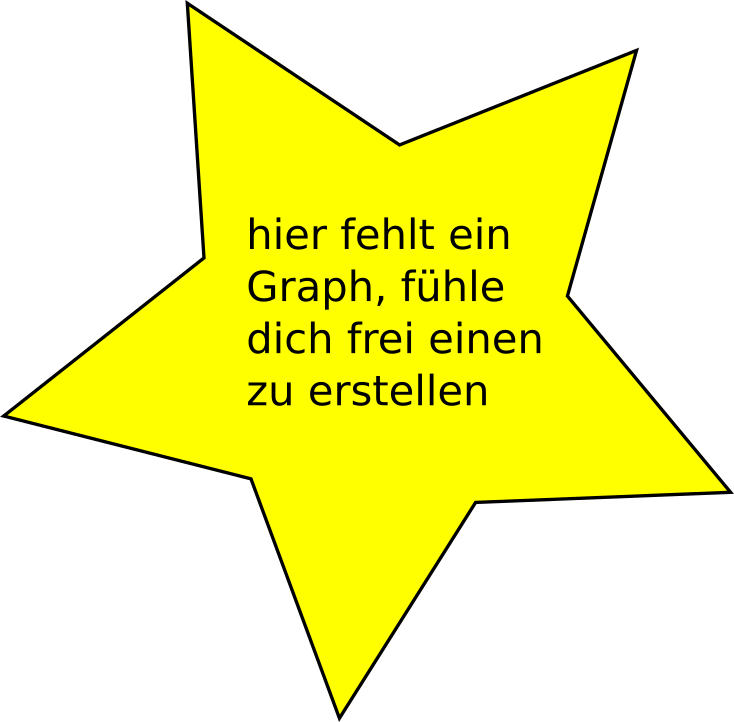
\includegraphics[width=0.7\linewidth]{graphs/dummy}
		%includegraphics{graphs/plot2.eps} \\
	\end{figure}

since $\epsilon$ is random, also $y$ is random with density $p(y|x, \Theta) - \frac{1}{\sqrt{2\pi}r} \exp (- \frac{\lVert y- \Theta^T x\lVert^2}{2r^2})$\\
To specify the model we have to estimate $\Theta \in \mathbb{R}^{n+1}$ from the data\\\\
idea: choose $\Theta$ that maximizes the likelihood\\\\
likelihood function:
\[L(\Theta) = \prod^m_{i=1} p(y^{(i)}|x^{(i)};\Theta)\]
the product form means: the observation $(x^{(1)},y^{(1)}), \dots , (x^{(i)}, y^{(i)})$ are independent of each other\\\\
estimate:
\[ \Theta_{ML} = \underset{\Theta \in \mathbb{R}^{n+1}}{argmax} L(\Theta) \]
\[ = \underset{\Theta \in \mathbb{R}^{n+1}}{argmax} \prod^m_{i=1} \frac{1}{\sqrt{2 \pi} \sigma} \exp \left(- \frac{(y^{(i)} - \Theta^T x^{(i)})^2}{2 \sigma^2}\right)\]
since we are only interested in the positoin where the maximum is attained we can apply a monoton transformation to $L(\Theta)$ with changing this position\\\\
$\Rightarrow \log$-likelihood function: $l(\Theta) = \log L(\Theta)$
\[ = \Theta_{ML} = \underset{\Theta \in \mathbb{R}^{n+1}}{argmax} l(\Theta)\]
\[ = \underset{\Theta \in \mathbb{R}^{n+1}}{argmax} \Sigma^m_{i=1} - \log (\sqrt{2\pi}\sigma) - \frac{1}{2\sigma}(y^{(i)} - \Theta^T x^{(i)})^2\]
\[\underset{\Theta \in \mathbb{R}^{n+1}}{argmax} - \textcolor{red}{m \log (\sqrt{2\pi}\sigma)} - \frac{1}{2\textcolor{blue}{\sigma^2}}\Sigma^m_{i=1}(y^{(i)} - \Theta^T x^{(i)})^2  \]
\begin{center}
\textcolor{red}{does not depend on $\Theta$}\space\space\space \textcolor{blue}{scaling vector does not influence the optimal $\Theta$}
\end{center}
\[ \underset{\Theta \in \mathbb{R}^{n+1}}{argmax} -\frac{1}{2} \Sigma^m_{i=1}(y^{(i)}-\Theta x^{(i)})^2\]
$X$: data matrix\\
$\Theta$: parameter vector\\
$Y$: response vector
\[\underset{\Theta \in \mathbb{R}^{n+1}}{argmax} -\frac{1}{2} \lVert X * \Theta - Y \lVert^2_2\]
\[ \underset{\Theta \in \mathbb{R}^{n+1}}{argmax} \textcolor{red}{\frac{1}{2} \lVert X * \Theta - Y \lVert^2_2}\]
\begin{center}
\textcolor{red}{$L(\Theta)$ loss function}\\
Minimizing the loss function that we discussed already\\
\end{center}
\end{enumerate}
\subsection*{remark} going non-linear $x \in \mathbb{R}, y \in \mathbb{R} \quad y=t(x)$
\begin{addmargin}[2 cm]{0 cm}
observations: $(x^{(1)}, y^{(1)}), \dots ,(x^{(i)}, y^{(i)}) \in \mathbb{R} \times \mathbb{R}$ but $f(.)$ not neccessarily linear function\\\\
$((x^{(1)},x^{(1)^2}, x^{(1)^3}), y^{(1)}), \dots , ((x^{(m)},x^{(m)^2}, x^{(m)^3}), y^{(m)})$\\
apply linear regression to argumented data points:\\\\
$\Rightarrow y = \Theta_0 + \Theta_1  x + \Theta_2  x^2 + \Theta_3 x^3$\\\\
linear regression gives \glqq good estimates\grqq\ for $\Theta_0, \Theta_1, \Theta_2, \Theta_3$\\\\
overfitting problem!

%TODO Hier einen entsprechenden Graphen einfügen
	\begin{figure}
		\centering
		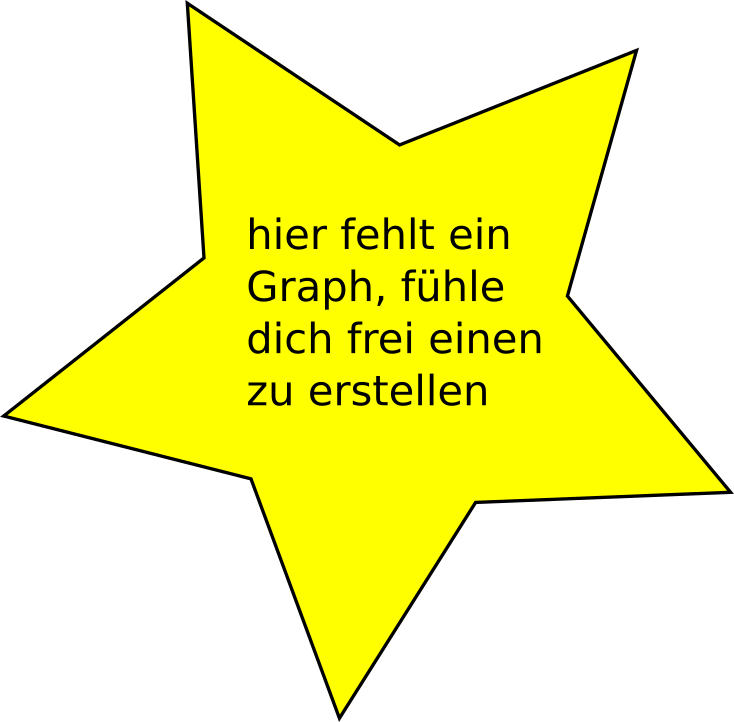
\includegraphics[width=0.7\linewidth]{graphs/dummy}
		%includegraphics{graphs/plot3.eps} \\
	\end{figure}
	
\end{addmargin}

\subsection*{logistic regression for binary classification}
data/observations: $(x^{(1)}, y^{(1)}), \dots , (x^{(i)}, y^{(i)})$\\\\
\begin{center}
 $x^{(i)} \in \mathbb{R}^n$ \space covariates\\
 $y^{(i)} \in {0,1}$ \space variates/response
\end{center}
probabilistic model of logistic regression
\[P[y=1|x;\Theta] = h_{\Theta}(x) \in (0,1)\]
\[P[y=0|x;\Theta] = 1-h_{\Theta}(x) \]

$h_{\Theta}(x) = g(\Theta^T x)$, where $g(.)$ is the logistic function $g(z) = \frac{1}{1+\exp(-z)}$\\\\
goal(as in linear regression): estimate $\Theta \in \mathbb{R}^n$ (Parameter vector) from data.\\
likelihood function for parameter vector $\Theta$:
\[L(\Theta) = \prod^m_{i=1} P[y^{(i)}|x^{(i)} ; \Theta]\]
again, assumption of independent observation
\[= \prod^m_{i=1} \textcolor{red}{h_{\Theta}(x^{(i)})^{y^{(i)}}} \textcolor{blue}{(1-h_{\Theta}(x^{(i)}))^{1-y^{(i)}}}\]
\begin{center}

$\textcolor{red}{=\begin{cases}1&\text{if $y^{(i)} = 0$}\\h_{\Theta}(x^{(i)})&\text{if $y^{(i)} = 1$}\end{cases}}$
$\textcolor{blue}{=\begin{cases}1&\text{if $y^{(i)} = 1$}\\1-h_{\Theta}(x^{(i)})&\text{if $y^{(i)} = 0$}\end{cases}}$\\
$\textcolor{red}{h_{\Theta} := P[y^{(i)} = 1 | x^{(i)};\Theta]}$\space\space
$\textcolor{blue}{1-h_{\Theta}(x^{(i)}) := P[y^{(i)} = 0 | x^{(i)};\Theta]}$
\end{center}

instead of working with the likelihood function it is easier to work with the $\log$-likelihood function:
\[\Theta_{ML} = \stackrel{argmax}{\Theta \in \mathbb{R}^n} L(\Theta) = \stackrel{argmax}{\Theta \in \mathbb{R}^n} \log \underbrace{L(\Theta)}_{\substack{l(\Theta)}}\]
\[= \stackrel{argmax}{\Theta \in \mathbb{R}^n} \Sigma^m_{i=1} y^{(i)} \log h_{\Theta}(x^{(i)}) + \underbrace{(1-y^{(i)}) \log(1-h_{\Theta}(x^{(i)}))}_{\substack{\log \text{likelihood function}}}\]
neccessary for optimum is a vanishing gradient\\
$\bigtriangledown_{\Theta} l(\Theta) \stackrel{!}{=}0$\\
for computing the gradient:
\[\frac{d}{dz} g(z) = \frac{d}{dz} \frac{1}{1+\exp(-z)}\]
\[= \frac{\exp(-z)}{(1+ \exp (-z))^2}\]
\[= \frac{1}{1+\exp (-z)} (\frac{1+\exp(-z) -1}{1+\exp(-z)})\]
\[= \frac{1}{1+\exp(-z)} (1-\frac{1}{1+\exp(-z)})\]
\[= \framebox{g(z)(1-g(z))}\]
\newline
\[\bigtriangledown_{\Theta} l(\Theta) = (\frac{\delta}{\delta \Theta_1} l(\Theta), \dots , \frac{\delta}{\delta \Theta_1} l(\Theta))\]
\[\frac{\delta}{\delta \Theta_j} l(\Theta)= \frac{\delta}{\delta \Theta_j} \Sigma^m_{i=1} y^{(i)}\log h_\Theta(x^{(i)}) + (1-y^{(i)}) \log (1-h_\Theta(x^{(i)}))\]
\[= \Sigma^m_{i=1} \left( \frac{y^{(i)}}{h_\Theta(x^{(i)})} - \frac{1-y^{(i)}}{1-h_\Theta(x^{(i)})}\right) \frac{\delta}{\delta\Theta_j} \underbrace{h_\Theta(x^{(i)})}_{\substack{g(\Theta^Tx^{(i)})}}\]
\[=\Sigma^m_{i=1} \left( \frac{y^{(i)}}{h_\Theta(x^{(i)})} - \frac{1-y^{(i)}}{1-h_\Theta(x^{(i)})}\right)\]
\[h_\Theta(x^{(i)})(1-h_\Theta(x^{(i)}))\underbrace{x^{(i)}_j}_{\substack{\text{j-th component i-th data vetor}}}\]
\[= \Sigma^m_{i=1} y^{(i)}(1-h_\Theta(x^{(i)}))-(1-y^{(i)})h_\Theta(x^{(i)})x^{(i)}_j\]
\[= \Sigma^m_{i=1}( y^{(i)}-h_\Theta(x^{(i)}))x^{(i)}_j\]
Unfortunetaly the system of equations $\frac{\delta}{\delta\Theta_j} l(\Theta)\stackrel{!}{=}0$ is highly non-linear and thus difficult to solve!
\[= \Sigma^m_{i=1}( y^{(i)}-h_\Theta(x^{(i)}))x^{(i)}_j = 0\]
turn to a numerical scheme(gradient ascend):\\\\
initialize: $\Theta^{(0)}$ arbitrary with some vector in $\mathbb{R}^n$\\
repeat
\begin{addmargin}[2 cm]{0 cm}
for $i=1$ to $m$
\begin{addmargin}[2 cm]{0 cm}
$\Theta_j^{(k)} = \Theta^{(k-1)}_j + \underbrace{\alpha}_{\substack{learning rate}} \Sigma^m_{i=1}(y^{(i)} - h_{\Theta^{(k)}} x^{(i)})x_j^{(i)}$
\end{addmargin}
end for
\end{addmargin}
until convergence
%bild

\section*{exercise 1 (08.04.2016)}

\begin{enumerate}[(1)]
\item
\[L(\Theta) = \frac{1}{2} \lVert X \Theta - Y \lVert^2_2 + \gamma \lVert \Theta \lVert^2_2 = \frac{1}{2} \Sigma^m_{i=1}(\underbrace{x^{(i)}\Theta}_{\substack{= \Sigma^n_{j=0} x^{(i)}_j \Theta_j}}-y^{(i)})^2 +\Sigma^n_{j=0} \Theta_j^2\]
\[= \frac{1}{2}\Sigma^m_{i=1}((\Sigma^n_{j=0} x_j^{(i)} \Theta_j)-y^{(i)})^2 +\gamma \Sigma^n_{j=0} \Theta_j^2\]
\[ \frac{\delta}{\delta\Theta_l}(\dots) = \Sigma^m_{i=1}((\Sigma^n_{j=0} x_j^{(i)} \Theta_j)-y^{(i)})x_l^{(i)} + 2 \gamma \Theta_l\]

\[\bigtriangledown_\Theta L(\Theta) = \underbrace{\frac{1}{2}\bigtriangledown_\Theta \lVert X \Theta-Y \lVert^2_2}_{\substack{= X^TX \Theta - X^TY}} + \underbrace{\gamma \bigtriangledown_\Theta \lVert \Theta \lVert^2_2}_{\substack{= 2 \gamma\Theta}}\]

\[= X^T X \Theta - X^TY + 2 \gamma \Theta \stackrel{!}{=} \Theta\]
\[\Rightarrow (X^TX + 2\gamma \mathds{1}) \Theta = X^T Y\]
\[\Rightarrow \Theta_{ridge} = (X^TX +2 \gamma \mathds{1})^{-1} X^TY \]
\begin{framed}
\[\lVert X \Theta -Y \lVert^2_2 = (X \Theta -Y)^T (X\Theta -Y)\]
\[= \Theta^T X^T X \Theta - \underbrace{\Theta^T X^T Y}_{\substack{(X\Theta)^T Y}} - \underbrace{Y^T X \Theta}_{\substack{Y^T (X\Theta) \Rightarrow -2 (X \Theta)^T Y = 2\Theta^T X^T Y = (X \Theta)^T Y}} + Y^T Y\]
\end{framed}
\item
Bayes: \[P(A|B) = \frac{P(AB)}{P(B)}\]
here: generative $\underbrace{\text{model}}_{\substack{\text{has parameters: $\phi, \Sigma, \mu_0, \mu_1$}}}$ that specifies how $y$ abd $x$ are generated\\\\
goal: estimate parameters from data $\rightarrow$ user likelihood function to do so
\[L(\phi,\Sigma,\mu_0, \mu_1) = \prod^m_{i=1} p(x^{(i)}, y^{(i)}; \phi,\Sigma,\mu_0, \mu_1)\]
\[\prod^m_{i=1} p(y^{(i)}, \phi) p(x^{(i)}; \Sigma, \mu_0)^{1-y^{(i)}} p(x^{(i)}; \Sigma, \mu_1)^{y^{(i)}}\]
\begin{framed}
\[p(x) = \frac{1}{\sqrt{2\pi} \sigma} \quad \exp \left( - \frac{(x-\mu)^2}{2 \sigma^2}\right)\]
density of 1-dim normal distribution $x \in \mathbb{R}$
\end{framed}

\begin{framed}
\[ p(x) = \frac{1}{(2\pi)^{\frac{n}{2}}} \underbrace{|\epsilon|^{\frac{n}{2}}}_{\substack{\sqrt{\det (\epsilon)} \quad \text{multi. var. extension of normal dist.}}}  \exp \left( - \frac{(x-\mu)^T \Sigma^{-1} (x-\mu)}{2} \right)\]
density of multi-variate distribution $x \in \mathbb{R}^n$
\end{framed}

parameters: $\underbrace{\mu \in \mathbb{R}^n}_{\substack{mem. vector}}, \Sigma \in \mathbb{R}^{n \times n}$\\
symmetric and positive definite (covariance matrix)\\\\
a matrix $\Sigma \in \mathbb{R}^{n \times n}$ is symmetric, if $\Sigma_{ij} = \Sigma_{ji} \forall i<j$\\
example: 
\[ \left( \begin{array}{ccc}
1 \quad 3 \\
3 \quad 2 \end{array} \right)\]
a symmetric matrix is called positive definite, if $x^T \Sigma x > 0$ for $x \neq 0$\\

example: data matrix $X \in \mathbb{R}^{m \times (n+1)}$
\[X^T X \in \mathbb{R}^{(n+1) \times (n+1)} (X^T X)_{ij} = x^{(i)^T}x^{(j)}\]
\[ = x^{(j)^T} x ^{(i)}\]
\[v^T(X^T X) = (Xv)^T (Xv)= \lVert Xv\lVert^2_2  \underbrace{\geq}_{\substack{\text{equality also allowed}}} 0 \quad\quad \text{positive semi-definite}\]
\end{enumerate}
loss function, eg. for logistic regression $L(\Theta)$
\[\Theta \in \mathbb{R}^{n+1} \rightarrow L(\Theta) \in \mathbb{R}, \text{that is, } L:\mathbb{R}^{n+1} \rightarrow \mathbb{R}\]
to get optimal $\Theta_i$ neccessary\\
$\bigtriangledown_\Theta L(\Theta) \stackrel{!}{=} 0$\\
vector with $(n+1)$ entries, we require that every entry is zero!

\section*{lecture 3 (11.04.2016)}
\subsection*{differentiability and convexiability}

Differentiability: function $t: \mathbb{R}^n \rightarrow \mathbb{R}, x \mapsto t(x)$\\
$t$ is differentiable at $x \in \mathbb{R}^n$ if $t$ can approximated well in x by a linear function.
\[\exists t'(x): t(y) = t(x) + \textcolor{red}{t'(x)^T} (y-x) + \textcolor{blue}{o(\lVert y-x\lVert)}\]
\begin{center}
\textcolor{red}{$\in \mathbb{R}^n$}\space\space\textcolor{blue}{little o-notation $\stackrel{lim}{r \rightarrow 0} \frac{1}{r} o(r) = 0$} 
\end{center}
not always possible:
%bild1
\subsection*{the gradient $t'(x)$ in coordinates}
using the definition of differentiability we can plug in special values for $y$.
\[y^{(i)}(t) = x + t\textcolor{red}{e_i}\]
\begin{center}
 \textcolor{red}{i-th standard basis vector $e_i = (0, \dots, 0,1,0, \dots ,0)^T, o(0)=0$ (the $1$ is position $i$)}
\end{center}
by differentiability we have:
\[t(y^{(i)}(t)) = t(x) + t'(x)^Ty^{(i)}(t) + o(\lVert y^{(i)}(t)-x\lVert)\]
\[= t(x) + tt'(x)^Te_i+o(t)\]
\[\Rightarrow t(y^{(i)}(t)) - t(x) - tt'(x)^Te_i = o(t)\]
\[\Rightarrow \frac{t(y^{(i)}(t))}{} - t'(x)^{T}e_i = \frac{1}{t} o(t)\]
\[\Rightarrow \textcolor{red}{\stackrel{lim}{t \rightarrow 0} \frac{t(y^{(i)}(t))}{t}} = \textcolor{blue}{t'(x)^Te_i}\]
\begin{center}
 \textcolor{red}{$= \frac{\delta t}{\delta x_i}(x)$ partial derivative}\space\space\textcolor{blue}{i-th component of the vector $t'(x)$ (gradient)}
\end{center}
\[\Rightarrow t'(x) = (\frac{\delta t}{\delta x_1}, \dots , \frac{\delta t}{\delta < n}(x))\]
generalization to functions $t: \mathbb{R}^n \rightarrow \mathbb{R}^m$\\
$t$ is called differentiable in $x \in \mathbb{R}^n$ if $\exists t'(x)\in\mathbb{R}^{m \times n} sit \forall y \in \mathbb{R}: t(y):$
\[ \underbrace{t(x)+t'(x)(y-x)}_{\substack{\text{linear approx.}}}+\underbrace{(|y-x|)}_{\substack{\text{vector little o-notation}}}\] 
here  $t'(x)$ is called Jacobi-Matrix\\\\

in coordinates:

\[ t'(x) =\left( \begin{array}{ccc}
\frac{\delta t_1}{\delta x_1} \dots  \frac{\delta t_1}{\delta x_n}\\
\vdots \quad \quad \quad \vdots\\
\frac{\delta t_m}{\delta x_1} \dots  \frac{\delta t_m}{\delta x_n} \end{array} \right)\] 


\[\lim_{v \rightarrow 0} \frac{1}{\lVert v \lVert} \quad o(v) = o \in \mathbb{R}^m \]
\[o(\underbrace{0}_{\substack{\in \mathbb{R}^m}})= 0\]
special case: assume, that $t: \mathbb{R}^n \rightarrow \mathbb{R}$ is differentiable in every $x \in \mathbb{R}^n$. That means $t'(x)$ exists for every $x \in \mathbb{R}^n$! Use this to define a new function:
\[t': \mathbb{R}^n \rightarrow \mathbb{R}^n , x \mapsto t'(x)\]
in coordiantes:

\[ t'(x) =\left( \begin{array}{ccc}
\frac{\delta^2 t}{\delta x_1 \delta_{x_1}}(x) \dots  \frac{\delta^2 t}{\delta x_n \delta_{x_1}}(x)\\
\vdots \quad \quad \quad \vdots\\
\frac{\delta^2 t}{\delta x_1 \delta_{x_n}}(x) \dots  \frac{\delta^2 t}{\delta x_n \delta_{x_n}}(x) \end{array} \right)\]

\subsection*{convex functions}
a subset $K \subset \mathbb{R}^n$ is called convex, if every $p,q \in K$ also $\lambda p + (1-\lambda) q \in K$ for $\lambda \in [0,1]$\\

%pic

a function $t:\mathbb{R}^n \rightarrow \mathbb{R}$ is called convex, if the epi-graph of the function 
\[epi(t) = \{(x,y) \in \mathbb{R}^{n+1} | y \geq f(x)\}\]
is a convex set

%pic

alternative characterization of convexity of functions:\\
$t: \mathbb{R}^n \rightarrow \mathbb{R}$ is convex, if for all $x,y \in \mathbb{R}^n$:
\[t(\lambda x + (1-\lambda)y) \leq \lambda t(x) + (1-\lambda) + t(x)\]

%pic
\begin{framed}
lemma: a differentiable function $t: \mathbb{R} \rightarrow \mathbb{R}$ is convex if and only if $t':\mathbb{R} \rightarrow \mathbb{R}$ ($x \mapsto t'(x)$) is increasing
\end{framed}

that is, it is enough to look at point $p,q \in \mathbb{R}^{n+1}$ that we on the boundary of the epi-graph of $t$

%proof

\begin{framed}
corrollary: a twice differentiable function is convex if its second derivative is always non-negative.\\
follows from: a differential function $t: \mathbb{R} \rightarrow \mathbb{R}$ is increasing if its derivative is non-negative
\end{framed}

\begin{framed}
theorem: a twice differential function $t: \mathbb{R}^n \rightarrow \mathbb{R}$ is convex, if and only if the hessian os positive semi-definite.

%proof
\end{framed}

\section*{lecture 4 (13.04.2016)}
\subsection*{characterization of convexity}
In terms of positivity of the hessian\\
$\rightarrow$ hessian is positive semi-definite everywhere\\\\
%bild
%bildcaption: lines of equal function values \glqq iso-lines \grqq
Linear regression is a convex optimization problem. Loss function of linear regression:
\[ L(\Theta) = \frac{1}{2} \lVert X \Theta Y \lVert^2_2\]
gradient of loss function:
\[\bigtriangledown_\Theta L(\Theta) = X^T X \Theta- X^T Y\]
To compute the hessian we need the derivative (jacobian) of
\[\underbrace{\Theta}_{\substack{\in \mathbb{R}^{n+1}}} \mapsto \bigtriangledown_\Theta L(\Theta) = X^T X \Theta- \underbrace{X^T Y}_{\substack{\text{does not depend on $\Theta$}}}, \quad\quad \in \mathbb{R}^{n+1}\]
$\rightarrow$ hessian of loss function:
\[\in \mathbb{R}^{(n+1)(n+1)}\]
\[X^T X = H_\Theta L(\Theta)\]
need to show $X^T X$ is positive semi-definite matrix $A \in \mathbb{R}^{(n+1)(n+1)}$ is called positive semi-definite if:
\begin{enumerate}[1.]
\item it is symmetric ($a_{ij} = a_{ji}$ for all indices)
\item $v^T Av \geq$ for all $v \in \mathbb{R}^{n+1}$
\end{enumerate}

$X^T X$:
\begin{enumerate}[1.]
\item symmetric, because $(X^T X)_{ij} = X^{(i)^T}X^{(j)}=X^{(j)^T}X^{(i)} = (X^T X)_{ij}$
\item positivity: $v^T X^T Xv: (Xv)^T(Xv) = \lVert Xv \lVert^2_2 \geq 0$
\end{enumerate}

\subsection*{remark}
\textbf{ridge regression}:
\[\bigtriangledown_\Theta k_{ridge}(\Theta) = X^T X \Theta - X^T Y + \gamma \mathds{1} \Theta, \quad\quad \underbrace{\gamma > 0}_{\substack{\text{regularization parameter}}}\]
\[\Rightarrow H_\Theta(l_{ridge}(\Theta)) = \underbrace{X^T X + \gamma \mathds{1}}\]
if $\gamma$ is large enough, the $X^T X +\gamma \mathds{1}$ is positive definite\\\\
$A \in \mathbb{R}^{(n+1)\times(n+1)}$ is called positive definite if,
\begin{enumerate}[1.]
\item $A$ is positive semi-definite
\item $v^T Av > 0$ for all $v \in \mathbb{R}^{n+1} \textbackslash \{0\} \quad\quad i.e. v \neq 0$\\
consequence of positive-definite hessian:

%2 bilder
%bild1caption: not strongly convex, minimum is not unique
%bild2caption: strongly convex
\end{enumerate}
\section*{exercise 2 (15.04.2016)}
\begin{enumerate}[(1)]
 \item likelihood Funktion: $L(\Theta) = \prod^m_{i=1} h_\Theta(x^{(i)}) (1-h_\Theta(x^{(i)}))^{1-y^{(i)}}$\\
 $h_\Theta(x) = \frac{1}{1+ \exp (- \Theta^T x)}$\\
 \textcolor{red}{ gesucht: $\Theta^k = \stackrel{argmax}{\Theta \in \mathbb{R}^n} l(\Theta) = \stackrel{argmax}{\Theta \in \mathbb{R}^n} \log L(\Theta) = \stackrel{argmax}{\Theta \in \mathbb{R}^n} \Sigma^m_{i=1} y^{(i)} \log h_\Theta(x^{(i)}) + (1-y^{(i)}) \log (1- h_\Theta(x^{(i)}))$}\\
 Ziel heute: Zeige, dass $l(\Theta)$ konkave Funktion ist, d.~h.
 \[l(\alpha \Theta_1 + (1- \alpha) \Theta_2) \geq \alpha l(\Theta_1) + (1-\alpha) l(\Theta_2)\]
\textcolor{red}{Es reicht zu zeigen, dass die Hesse-Matrix von $l(\Theta)$ negativ semidefinit ist.}

%bild
\begin{framed}

\[g(\epsilon) \frac{1}{1+\exp(-\epsilon)} \in (0,1) \quad\quad \text{logistische Funktion}\]
\[\frac{d_g(t)}{dt} = \frac{1}{(1+ \exp (-t))}^2 - \exp(-t) = \frac{1}{1+\exp (-t)} \left(1- \frac{1}{1+\exp (t)}\right)\]
\[g(t)(1-g(t))\]
\[\Rightarrow \frac{\delta h_\Theta(x)}{\delta \Theta_j} = h_\Theta(x)(1-h_\Theta(x)) \frac{\delta}{\delta \Theta_j} \Theta^T x\]
\[= h_\Theta(x)(1-H_\Theta(x))x_j\]
\begin{framed}
Kettenregel
\[h_\Theta(x) = g(\Theta^T x)\]
\[\underbrace{x}_{\substack{\in \mathbb{R}^n}} \underbrace{\mapsto}_{\substack{\text{innere Fkt.}}} \underbrace{\Theta^T}_{\substack{\in \mathbb{R}^n x}} \underbrace{\mapsto}_{\substack{\text{äußere Fkt.}}} \underbrace{g(\Theta^T x)}_{\substack{\in \mathbb{R}^n}}\]
\[\frac{\delta}{\delta \Theta_j} \Theta^T x = \frac{\delta}{\delta\Theta_j}(\Sigma^m_{i=0} \Theta_i x_i) = \frac{\delta}{\delta\Theta_j}(\Theta_1 x_1 + \Theta_1 x_1 + \dots + \Theta_n  x_n) = x_j\]
\end{framed}
\end{framed}


Wir wissen schon: 
\[ \frac{\delta l(\Theta)}{\delta \Theta_j} = \Sigma^m_{i=1}(\underbrace{y^{(i)}}_{\substack{\in \{0,1\}}} - \underbrace{\Theta(x^{(i)}))}_{\substack{\in (0,1)}} x^{(i)}_j\]
\[ \frac{\delta^2 l(\Theta)}{\delta \Theta_k \delta \Theta_j} = \frac{\delta}{\delta \Theta_k }\Sigma^m_{i=1} (y^{(i)} - h_\Theta(x^{(i)})) x_j^{(i)}\]
\[ =\underbrace{\frac{\delta}{\delta \Theta_k} (\Sigma_{i=1}^m y^{(i)} x_j^{(i)})}_{\substack{= 0, \text{hängt nicht von $\Theta$ ab}}} - \frac{\delta}{\delta \Theta_k} (\Sigma^m_{i=1} h_\Theta(x^{(i)}) x_j^{(i)})\]
\[ = \frac{\delta}{\delta \Theta_k} \Sigma^m_{i=1} h_\Theta (x^{(i)}) x_j^{(i)}\]
\[ = - \Sigma^m_{i=1} \frac{\delta}{\delta \Theta_k} (h_\Theta(x^{(i)}) x_j^{(i)})\]
\[ = - \Sigma^m_{i=1} x_j^{(i)} \frac{\delta}{\delta\Theta_k} h_\Theta(x^{(i)})\]
\[ = - \Sigma^m_{i=1} \underbrace{h_\Theta(x^{(i)})}_{\substack{> 0}} \underbrace{(1- h_\Theta(x^{(i)}))}_{\substack{> 0}} x_j^{(i)} x_k^{(i)}\]
Wir müssen zeigen, dass $v^T \quad H(\Theta)v \geq 0$ für alle $v \in \mathbb{R}^n$
\[ \underbrace{H(\Theta)}_{\substack{\in \mathbb{R}^{n \times n}}} = (H_{kj}(\Theta)) = \left( \frac{\delta^2 l(\Theta)}{\delta\Theta_k \delta\Theta_j}\right)\]

%Ich hoffe, dass es ab hier auch wirklich so weiter ging
$H(\Theta)$ ist symmetrisch, da
\[H_{kj}(\Theta) = - \Sigma^m_{i=1} h_\Theta (x^{(i)})(1-h_\Theta (x^{(i)})) x_j^{(i)} x_k^{(i)}\]
\[= - \Sigma^m_{i=1} h_\Theta(x^{(i)})(1-h_\Theta(x^{(i)})) x_k^{(i)}x_j^{(i)}\]
\[= H_{jk}(\Theta) = x_j\]
negativ semi-definit
\[H(\Theta) = - \Sigma^m_{i=1} h_\Theta(x^{(i)})(1-h_\Theta(x^{(i)})) \underbrace{x^{(i)}x^{(i)^T}}\]
\begin{center}
äußeres Produkt des i-ten Datenvektors mit sich selbst
\end{center}
Bsp. Äußeres Produkt:
\[x = \left( \begin{array}{ccc} x_1 \\ x_2 \end{array} \right), \quad x x^T = \left( \begin{array}{ccc} x_1 \\ x_2 \end{array} \right) (x_1 x_2) \]
\[= \left( \begin{array}{ccc} x_1x_1 \quad x_1x_2 \\ x_2x_1 \quad x_2x_2 \end{array} \right) = \left( \begin{array}{ccc} x_1^2 \quad x_1x_2 \\ x_2x_1 \quad x_2^2 \end{array} \right)\]
\[ = \left( \begin{array}{ccc} x_1^2 \quad x_1x_2 \\ x_1x_2 \quad x_2^2 \end{array} \right)\]
\begin{enumerate}[(1)]
\item äußeres Produkt ist symmetrische Matrix
\item äußeres Produkt ist semi-definit
\end{enumerate}
\[v^T (x x^T)v\]
\[= (v^T)(x^T v)\]
\[= (v^T)(v^T x)\]
\[(v^T x)^2 \geq 0\]
\begin{center}
$xx^T$ aus Abbildung $\mathbb{R}^n \mapsto \mathbb{R}^n$\\
$v \mapsto (xx^T)v = x(v^Tx)$
\end{center}

\subsection*{Statistische Modelle}
\begin{enumerate}[1.]
\item lineare Regression: \[p(y,x) = \frac{1}{\sqrt{2 \pi} \sigma} \exp(- \frac{\lVert y- \Theta^T x \lVert^2_2}{2 \sigma^2})\]
\item logistische Regression: \[P[y=1;x] = h_\Theta(x)\]
\[P[y=0;x] = 1-h_\Theta(x)\]
\end{enumerate}

$h_\Theta(x) = \frac{1}{1+\exp(-\Theta^T x)}$ benutzt logistische Funktion $g(z) = \frac{1}{1+\exp(-z)}$
1,2 sind konditionale Modelle, d.h. nur $y$ ist zufällig\\
$y \in \mathbb{R}$ (lineare Regression)\\
$y \in \{0,1\}$ (logistische Regression)\\
$\Rightarrow x$ frei wählbar, Messung von $y$ an der Stelle $x$ ist Zufallsexperiment

\begin{enumerate}
\item[3.] Gauss'sche Diskriminanzanalyse (Klassifikation)
\item[4.] Naive Bayes (Kontingenzanalyse)
\end{enumerate}

3,4 sind generative Modelle, d.h. sowohl $x$ als auch $y$ sind zufällig
\item Likelihood-Funktion der Gauss'schen Diskriminanzanalyse
\[L(\phi,\mu_0, \mu_1, \Sigma) = \prod^m_{i=1} p(x^{(i)},y^{(i)};\phi,\mu_0, \mu_1, \Sigma\]
\[\phi \in [0,1], \quad\quad \mu_0, \mu_1 \in \mathbb{R}^n, \quad\quad \Sigma \in \mathbb{R}^{n \times n} \text{positiv definit}\]
\[\text{Datenpunkte: } (x^{(1)},y^{(1)}, \dots , x^{(m)},y^{(m)})\]

\begin{framed}
Erinnerung: Likelihood-Funktion für logistische Regression:
\[L(\Theta) = \prod^n_{i=1} P[y^{(i)} | x^{(i)}, \Theta]\]
\end{framed}

\begin{framed}
Unterscheidung:
\begin{enumerate}[1.]
\item Zufallsvariable $x$ nimmt nur endlich viele Werte $\{1, \dots , k\}$ an. Dann kann $x = i$ eine Wahrscheinlichkeit $P[x = i]$ zuordnen.
\item Zufallsvariable $x$ nimmt Werte in $\mathbb{R}$ an. Dann kann man den Ereignissen $X \in [a,b]$ eine Wahrscheinlichkeit zuordnen $P[X \in [a,b]] = \int^b_a p(x) dx$. Dabei ist $p:\mathbb{R} \rightarrow \mathbb{R}$ eine Wahrscheinlichkeitsdichte, d.h.

\begin{enumerate}[(1.)]
\item $\int^\infty_{- \infty} p(x) dx = 1$
\item $p(x) \geq 0$
\end{enumerate}
\end{enumerate}
\end{framed}

\begin{framed}
 Bayes Theorem:
 \[p(x|y) = \frac{p(x,y)}{p(y)}\]
 \[\Rightarrow p(x,y) = p(x|y)p(y)\]
\end{framed}
\[= \prod^m_{i=1} p(x^{(i)} | y^{(i)} ; \mu_0, \mu_1, \Sigma) P(y^{(i)}; \phi)\]
\[= \prod^m_{i=1} p(x^{(i)} | y^{(i)} = 1; \mu_0, \Sigma)^{y^{(i)}} p(x^{(i)} | y^{(i)} = 0 ; \mu_1, \Sigma)^{1-y^{(i)}}\]
\[= \left( \frac{1}{(2\pi)^{\frac{a}{2}}} |\Sigma|^{\frac{1}{2}}\right)^m \prod^m_{i=1} \exp(- \frac{1}{2}) (x^{(i)} \mu_1)^T \Sigma^{-1} (x^{(i)} - \mu_1))^{1-y^{(i)}} \exp(- \frac{1}{2}(x^{(i)} - \mu_0)^T \Sigma^{-1}(x^{(i)}-\mu_0))^{1-y^{(i)}}\]
\[ \dots \phi^{y^{(i)}}(1-\phi)^{1-y^{(i)}}\]

Notationeller Trick:
\[a^{y^{(i)}} = a^{\tilde{x}_{\{y^{(i)} = 1\}}}\]
\[\tilde{x}_{\{y^{(i)} = 1\}} = =\begin{cases}1&1, \text{falls } y^{(i)} = 1\\2&0, \text{falls } y^{(i)} = 0\end{cases}\]

\[= \left( \frac{1}{(2\pi)^{\frac{a}{2}}} |\Sigma|^{\frac{1}{2}}\right)^m \prod^m_{i=1} \exp (- \frac{1}{2} (x^{(i)} - \mu_1)^T \Sigma^{-1} (x^{(i)} - \mu_1))^{\tilde{x}_{\{y^{(i)} = 1\}}} * \]
\[\exp (- \frac{1}{2} (x^{(i)} - \mu_0) \Sigma^{-1} (x^{(i)} - \mu_0 ))^{\tilde{x}_{\{y^{(i)} = 0\}}} * \dots *\]
\[\phi^{y^{(i)}} (1-\phi^{1-y^{(i)}})\]
\end{enumerate}

Merkregel: Die Likelihood-Funktion ist die Wahrscheinlichkeit der Beobachtungen als Funktion der Parameter.\\
Da es einfach ist, mit Summen als mit Produkten zu arbeiten: Übergang zur $\log$-Likelihood-Funktion
\[ l (\phi, \mu_0, \mu_1, \Sigma) = \log L(\phi, \mu_0, \mu_1, \Sigma)\]
\[= -m \log ((2\pi)^{\frac{n}{2}} |\Sigma|^{\frac{1}{2}})\]
\[- \Sigma^n_{i=1} \tilde{x}_{\{y^{(i)} = 1\}} (x^{(i)} - \mu_1)^T \Sigma^{-1} (x^{(i)}-\mu_0)\]
\[- \Sigma^n_{i=1} \tilde{x}_{\{y^{(i)} = 0\}} (x^{(i)} -\mu_0)^T \Sigma^{-1} (x^{(i)} - \mu_1)\]
\[+ \Sigma^m_{i=1} (y^{(i)} \log \phi + (1-y^{(i)}) \log (1-\phi))\]
Für die max. Likelihood-Schätzung von $\phi$, d.h. bestimme desjenigen $\phi$, das $\log$-Likelihood-Funktion maximiert. Notwendig, dass Ableitung nach $\phi$ verschwindet.
\[\frac{d l(\phi,\mu_0,\mu_1,\Sigma)}{d\phi} = \Sigma^m_{i=1} \frac{y^{(i)}}{\phi} - \frac{(1-y^{(i)})}{1-\phi} \stackrel{!}{=} 0\]
\[\Rightarrow (1-\phi) \Sigma^m_{i=1} y^{(i)} \stackrel{!}{=} \phi \Sigma^m_{i=1} 1-y^{(i)} \Rightarrow \Sigma^m_{i=1} 1 = m_i \phi\]
%bei m_i \phi bin ich mir nicht sicher! Bitte nochmal drübersehen
\begin{framed}
\[\Rightarrow \phi = \frac{1}{m} \Sigma^m_{i=1} y^{(i)}\]
\begin{center}
Max. Likelihood-Schätzung für $\phi$
\end{center}
\end{framed}

Maximierung der Likelihood-Schätzung von $\mu_1$. Beachte: $\mu_1 \in \mathbb{R}^n$. Notwendig für Maximum der $\log$-Likelihood-Funktion ist das Verschwinden des Gradienten nach $\mu_1$.
\[\bigtriangledown_{\mu_1} l(\phi, \mu_0, \mu_1, \Sigma) = \bigtriangledown_{\mu_0} (- \frac{1}{2} \Sigma^m_{i=1} \tilde{x}_{\{y^{(i)} = 1\}} (x^{(i)}-\mu_1)^T \Sigma^{-1} (x^{(i)} - \mu_1))\]
\[= - \frac{1}{2} \Sigma^m_{i=1} \tilde{x}_{\{y^{(i)} = 1\}} \bigtriangledown_{\mu_1}\]
\[(\underbrace{(x^{(i)} - \mu_1)^T \Sigma^{-1} (x^{(i)} - \mu_1)}_{\substack{= x^{(i)} \Sigma^{-1} x^{(i)} -2\mu_1^T \Sigma^{-1} x^{(i)} + \mu_1^T \Sigma^{-1}}})\]
\[= - \frac{1}{2} \Sigma^m_{i=1} \tilde{x}_{\{y^{(i)} = 1\}} (-2 \Sigma^{-1} x^{(i)} + 2 \Sigma^{-1} \mu_1)\]
\[\Sigma^m_{i=1} \tilde{x}_{\{y^{(i)} = 1\}} \Sigma^{-1} \mu_1 - \Sigma^{-1} x^{(i)}\]
\[\Sigma^m_{i=1} \tilde{x}_{\{x^{(i)} = 1\}} \Sigma^{-1} (\mu_1 - x^{(i)})\]
\[\Sigma^{-1} (\Sigma^m_{i=1} \tilde{x}_{\{y^{(i)} = 1\}} (\mu_1 - x^{(i)})) \stackrel{!}{=} 0\]

\begin{framed}
Erinnerung: $\Sigma$ ist positiv definit
\begin{itemize}
\item $\Rightarrow \Sigma$ ist invertierbar
\item $\Rightarrow \Sigma^{-1}$ ist invertierbar 
\end{itemize}
\[\Sigma\Sigma^{-1} = \Sigma^{-1}\Sigma = \mathds{1}_n = \left( \begin{array}{ccc} 1 \quad\quad 0 \\ \ddots \\ 0 \quad\quad 1 \end{array}\right) \in \mathbb{R}^{n \times n}\]
\end{framed}
Situation:
\[\Sigma^{-1} v = 0\]
\[\Rightarrow \Sigma\Sigma^{-1} v = \Sigma * 0 = 0\]
\[\mathds{1}_n v = 0\]
\[\Rightarrow v = 0\]
Hier:
\[v = \Sigma^m_{i=1} \tilde{x}_{\{y^{(i)}= 1\}} (\mu_1 - x^{(i)})\]
\[\Rightarrow \Sigma^m_{i=1} \tilde{x}_{\{y^{(i)}=1\}} (\mu_1 - x^{(i)}) = 0\]
\[\Rightarrow \mu_1 \Sigma^m_{i=1} \tilde{x}_{\{ y^{(i)} = 1\}} = \Sigma^m_{i=1} \tilde{x}_{\{y^{(i)}=1\}} x^{(i)}\]
\begin{framed}
\[\Rightarrow \mu_1 = \frac{\Sigma^m_{i=1}\tilde{x}_{\{y^{(i)}=1\}} x^{(i)}}{\Sigma^m_{i=1}\tilde{x}_{\{y^{(i)}=1\}}}\]
\begin{center}
Maximierung der Likelihood-Schätzung von $\mu_1$
\end{center}
\end{framed}
Analog (Symmetrie):
\begin{framed}
\[\Rightarrow \mu_1 = \frac{\Sigma^m_{i=1}\tilde{x}_{\{y^{(i)}=0\}} x^{(i)}}{\Sigma^m_{i=1}\tilde{x}_{\{y^{(i)}=0\}}}\]
\begin{center}
Maximierung der Likelihood-Schätzung von $\mu_0$
\end{center}
\end{framed}



\section*{Lecture 6 (20.04.2016)}
	\subsection*{Gauss'sche Diskriminanzanalyse}
		\subsubsection*{Bisher:}
			Maximum Likelihood-Schätzung der Parameter $\phi, \mu _0 \mu _1$
			
			\textcolor{red}{Eigentlich $\Sigma$ schätzen, das ist etwas aufwändiger}
			\textcolor{red}{\[ \Sigma _{ML} = \sum_{i=1}^{m} \chi_{\{y^{(i)} = 1\}} (x^{(i)} - \mu_0) (x^{(i)} - \mu_1)^T + \sum_{i=1}^{m} \chi_{\{y^{(i)} = 0\}} (x^{(i)} - \mu_0) (x^{(i)} - \mu_1)^T \quad   \footnote{$(x^{(i)} - \mu_0) (x^{(i)} - \mu_1)^T$ ist Rang 1 Matrix}\]}
			
		\subsubsection*{Wichtig:}
			$\Sigma$ ist gleich für die beiden Klassen $y = 1$ bzw. $y = 0$.
			
		\subsubsection*{Jetzt:}
			Bestimmung der Entscheidungsgrenze
			\[x: P[y = 1 | x] = P[y = 0 | x]  \textcolor{red}{= \frac{1}{2}} \quad \footnote{$ x \in \mathbb{R} $}\]
		\subsubsection*{Hinweis:}
			Zeige, dass
			\begin{gather*}
				P[y = 1 | x]  = \frac{1}{1 + \exp(- \Theta ^T x)} \\
				\Rightarrow P[y = 0 | x]  = 1 - \frac{1}{1 + \exp(- \Theta ^T x)}
			\end{gather*}
%			\hskip
			
			 \textcolor{red}{Sieht aus wie die logistische Regression ist aber anders: 				
				\begin{enumerate}
					\item Generatives vs. Diskriminierendes Modell
					\item $ \Theta $ bei logistischer Regression ist allgemeiner
				\end{enumerate}
			}
			
		\subsubsection*{Aufgabe:}
			Umformen von
			%TODO footnote wird nicht angezeigt -> keine Fußnoten innerhalb Umgebung 
			\begin{gather*}
				P[y = 1 | x]  = \frac{p(y = 1,x )}{p(x)} \\
%				
				= \frac{p(x|y=1)P[y=1]}{p(x|y=)P[y=0] + p(x|y=1)P[y=1]} \quad \footnote{$ P[y=1] = \phi $} \footnote{$ P[y=0] = 1- \phi $} \\
%				
				= \frac{\phi \exp(-\frac{1}{2}(x-\mu_1)^T \Sigma^{-1} (x-\mu_1))}{(1 - \phi ) \exp(-\frac{1}{2}(x-\mu_0)^T \Sigma^{-1} (x-\mu_0)) + \phi \exp(-\frac{1}{2}(x-\mu_1)^T \Sigma^{-1} (x-\mu_1))} \\
%
				= \frac{1}{(\frac{1 - \phi }{\phi}) \exp(-\frac{1}{2}(x-\mu_0)^{T}  \Sigma^{-1} (x-\mu_0) + \frac{1}{2}(x-\mu_1)^T \Sigma^{-1} (x-\mu_1)) + 1} \quad \footnote{$ \frac{1}{exp(-a)} = \exp(a)  $ \\
					$ \frac{\exp(a)}{\exp(b)} = \exp(a - b) $} \footnote{NR: $ (x-\mu_0)^T \Sigma^{-1} (x-\mu_0) = x^T \Sigma^{-1} x - 2\mu_0^T \Sigma^{-1} x  + \mu_0^T \Sigma^{-1} \mu_0 $}\\
%					
				= \frac{1}{(\frac{1 - \phi }{\phi}) \exp(-2(\mu_0 - \mu_1)^{T}  \Sigma^{-1} x - \mu_0^T \Sigma^{-1} \mu_0 + \mu_1^T \Sigma^{-1} \mu_1) + 1} \\
%				 
				= \frac{1}{\exp(-2(\mu_0 - \mu_1)^{T}  \Sigma^{-1} x - \mu_0^T \Sigma^{-1} \mu_0 + \mu_1^T \Sigma^{-1} \mu_1 + log(1- \phi) - log(\phi) + 1} \\
%				
				= \frac{1}{\exp(- \Theta^Tx)+1}
			\end{gather*}
			
			%TODO footnote wird nicht angezeigt -> keine Fußnoten innerhalb Umgebung
			\begin{gather*}
				x = (1,x_1,\dots,x_n) \in \mathbb{R}^{n+1}\\
%				
				\Theta_0 = \mu_0^T \Sigma^{-1} \mu_0 - \mu_1^T \Sigma^{-1} \mu_1 - log(1- \phi) + log(\phi) \\
%				
				\Theta_i = (2(\mu_0 - \mu_1)^T \Sigma^{-1})_i \quad \footnote{Vektor in $ \mathbb{R}^n $, i-te Koordinate des Vektors}
			\end{gather*}
			
			\begin{gather*}
				P[y = 0 | x] = 1 - P[y = 1 | x]  = 1 - \frac{1}{1 + \exp(- \Theta^Tx)} \\
				= \frac{\exp(- \Theta^Tx)}{1 +\exp(- \Theta^Tx)} \\
				= \frac{1}{\exp( \Theta^Tx) + 1} \\
				= \frac{1}{1+ \exp(\Theta^Tx)}
			\end{gather*}
		
		\subsubsection*{Bestimmung der Entscheidungsgrenze:}
			
			%TODO footnote wird nicht angezeigt -> keine Fußnoten innerhalb Umgebung
			\begin{gather*}
				x : P[y = 1 | x] = P[y = 0 | x] \\
				\Leftrightarrow x : \frac{1}{1+ \exp(- \Theta^Tx)} = 1 - \frac{1}{1+ \exp(- \Theta^Tx)} \\
				\Leftrightarrow x : \frac{2}{1+ \exp(- \Theta^Tx)} = 1 \\
				\Leftrightarrow x : 2 = 1 + exp(- \Theta^Tx) \\
				\Leftrightarrow x : 1 = exp(- \Theta^Tx) \\
				\Leftrightarrow x : 0 = - \Theta^Tx \quad \footnote{Ziehen des Logarithmus} \\
				\Leftrightarrow x : 0 = \Theta^Tx 				
			\end{gather*}
			
		\subsubsection*{Entscheidungsgrenze:}
		
			\[ \{x \in \mathbb{R}^n | \Theta^Tx + \Theta_0 = 0 \} \]
		
			 Wie sieht die Entscheidungsgrenze Geometrisch aus? \\
			Fall $ \Theta_0 = 0: x: \Theta^Tx = 0$ \medskip \footnote{D.h. x muss senkrecht zum Vektor $ \Theta $ sein $ \Rightarrow $ Entscheidungsgrenze ist ein $ n-1 $- Dimensionaler Unterraum des $ \mathbb{R}^n $}
			
			%TODO Plot muss erstellt werden
			\begin{figure}
				\centering
				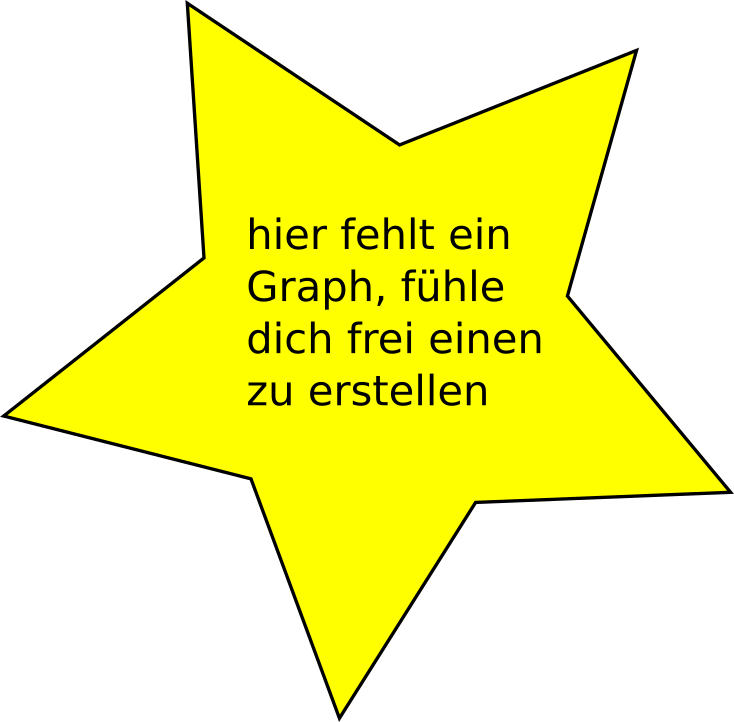
\includegraphics[width=0.7\linewidth]{graphs/dummy}
%				\includegraphics[width=0.7\linewidth]{graphs/plot6_1}
				\caption{Entscheidungsgrenze wird durch einen Eindimensionalen Unterraum othogonal zu $ \Theta $}
			\end{figure}
			
			 Fall $ \Theta_0 \neq 0 \Rightarrow$ Verschiebung des $ (n-1) $- Dimensionalen Unterraums
			
			%TODO Plot muss erstellt werden
			\begin{figure}
				\centering
				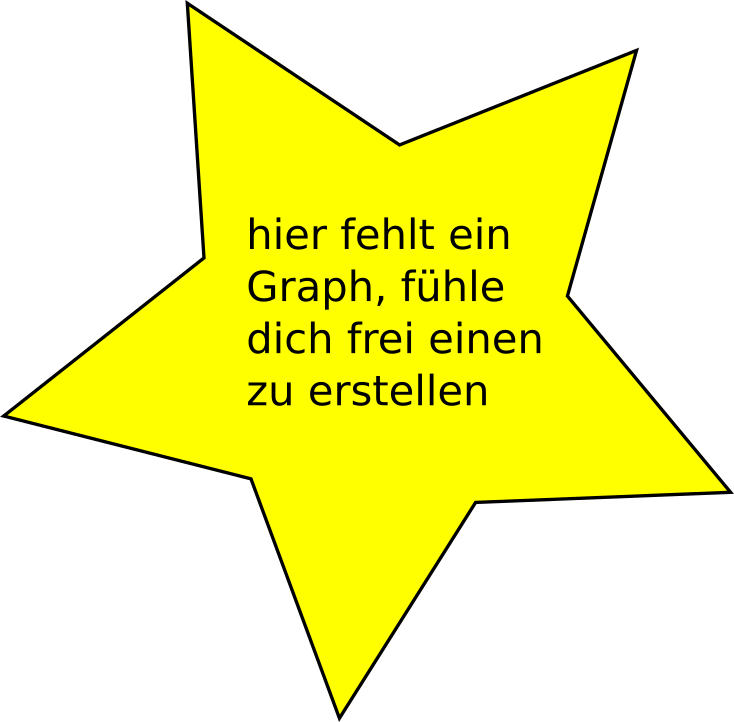
\includegraphics[width=0.7\linewidth]{graphs/dummy}
%				\includegraphics[width=0.7\linewidth]{graphs/plot6_2}
				\caption{a : Abstand des Unterraums zum Ursprung}
			\end{figure}
			
			\subsubsection*{Einschub vektorisierte Schreibweise}
			 log-Likelihood Funktion für ligistische Regression:
			
			\[ l(\Theta) = \sum_{i = 1}^{m} y^{(i)} \log h_\Theta (x^{(i)}) + (1 - y^{(i)}) \log(1 - h_\Theta x^{(i)})\]
			\[ h_\Theta (x^{(i)})  = \frac{1}{1 + \exp(- \Theta^T x^{(i)})}\]
			
			 Vektorisieren:
			
			\[Datenmatrix \quad	X = 
				\begin{matrix} \begin{pmatrix} x^{(1)^T} \\ \vdots \\ x^{(m)^T}	\end{pmatrix}  \end{matrix}
				\begin{matrix} \begin{pmatrix} x_1^{(1)} & \dots & x_n^{(1)} \\ \vdots & \ddots & \vdots \\ x_1^{(m)}	& \dots & x_n^{(m)}\end{pmatrix}  \end{matrix} \]
				
			\[ vec(a) * (y*.log.(vec(1)/. (vec(1) +. exp.(-x \cdot \Theta))))  \textcolor{red}{ = \sum_{i = 1}^{m} y^{(i)}\log(h_\Theta(x^{(i)}))}\]
			
			\subsection*{3. Einführungsbeispiel \small{(1. Lineare Regression, 2. Logistische Regression)}}
			
			Das Naive Bayes Verfahren (Hier als Beispiel für eine Kontingenzanalyse)
			
			\subsubsection*{Daten:}
				\[ (x^{(1)}, y^{(1)}), \dots, (x^{(m)}, y^{(m)}) \]
				\begin{gather*}
					y^{(i)} \in \{0,1\} \quad Variates
					x^{(i)} \in \{0,1\}^n \quad Covarates 
				\end{gather*}
				
				
			\subsubsection*{Modell:}
				%TODO Fußnote wird nicht angezeigt
				\begin{gather*}
					P[y =1] = \Theta_y, P[y =0] = 1 - \Theta_y \\
					P[x|y] = P[x_1,\dots,x_n|y] =\footnote{Naive Bayes Annahme} = \prod_{i = 1}^{n} P[x_i|y] \\
					= \prod_{i = i}^{n} [ \Theta_{x_i,y=1} ^{x_i} (1- \Theta_{x_i, y = 1})^{1-x_i}]^y [ \Theta_{x_i,y=0} ^{x_i} (1- \Theta_{x_i, y = 0})^{1-x_i}]^{1-y}
				\end{gather*}
			
			\subsubsection*{\textcolor{red}{Modellparameter}}
				
				\textcolor{red}{\[ \Theta_y, \Theta_{x_i,y = 1} (i=1,\dots,n), \Theta_{x_i,y = 0} (i=1,\dots,n)  \Rightarrow 2n + 1 \medspace Parameter\]}
			
			 [Im ganz allgemeinen Modell haben wir $ 2^{n+1}-1 $ Parameter]
			

\section*{exercise 3 (22.04.2016)}

\paragraph{Naive Bayes}

\subsection*{Wiederholung Bayes Modell}
\begin{tabular}{lll}
variate   & \{0,..,1\}   & \{0,..,k\}   \\
covariate & \multicolumn{2}{l}{\{0,1\}}
\end{tabular}

Modell: 
\begin{enumerate}
\item \[ P[y=1] = \phi\]  \[ P[y=0] = 1 - P[y=1] = 1 - \phi \]
\item \[ P[x|y=1] = P[x_1,...,x_n | y] = \leftarrow \footnote{hier eine naive Annahme, dass alle $x$ von einander unabhängig sind.}\]   \\
\[ = \prod_{i=1}^n P[x_i | y=1] = \prod_{i=1}^n \phi_{x_i = 1, y = 1}^{x_i} (1 - \phi_{x_i = 1, y = 1})^{1 - x_i} \] \\
Analog: \[ P[x|y=0] = \prod_{i=1}^n P[x_i | y = 0] = \prod_{i=1}^n \phi_{x_i = 1, y = 0}^{x_i} (1 - \phi_{x_i = 1, y = 0})^{1 - x_i}\]
\end{enumerate}

\textcolor{blue}{Modell Parameter: \[ \phi, \phi_{x_i = 1, y = 1} , \phi_{x_i = 1, y = 0} \] insgesamt $2n + 1$ Parameter.}\\

Schätzten der Parameter aus den Daten: $(x^{(1)},y^{(1)}),...,(x^{(n)},y^{(n)})$.\\
Dazu verwende Likelihood-Funktion: \\
\[L(\phi, \phi_{x_i,y=1}, \phi_{x_i,y=0}) = \prod_{i=1}^{m} P[x^{(i)},y^{(i)}] = \]
\[ = \prod_{i=1}^{m} P[x^{(i)}|y^{(i)}] \cdot P[y^{(i)}] = \]

%TODO Den Teil >> \cdot \phi^{y^{(i)}} \cdot (1 - \phi)^{1 - y^{(i)}} << am Schluss habe ich nicht in meinen Unterlagen -Sascha
\[ \prod_{i=1}^{m} \prod_{j=1}^{n} [\phi_{x_{j}^{(i)},y^{(i)}=1} ^{x_j} \cdot (1 - \phi_{x_{j}^{(i)},y^{(i)}=1}^{x_j})^{1 - x_{j}^{(i)}} ]^{y^{(i)}} [\phi_{x_{j}^{(i)},y^{(i)} =0} ^{x_j} \cdot (1 - \phi_{x_{j}^{(i)},y^{(i)}=0}^{x_j})^{1 - x_{j}^{(i)}}]^{1-y^(i)} \cdot \phi^{y^{(i)}} \cdot (1 - \phi)^{1 - y^{(i)}} \]   


\subsection*{Aufgabe }

Schätze \[ \phi und \phi_{x_j,y=1} \]

\[ \phi_{ML} = \frac{1}{m} \cdot \sum_{i=1}^{m} y^{(i)} \]\footnote{Intuitiv und wie bei gaußscher Diskriminanzanalyse}
\footnote{ML steht hier für Maximum-Likelihood} \\

\[ \phi_{x_j,=1}^{ML} = \frac{\sum_{i=1}^{m} y^{(i)}x_{j}^{(i)} }{\sum_{i=1}^{m} y^{(i)}} \] [Aus den Experimenten/E-mails betrachten wir nur die jenigen, wo \[ y^{(i)} = 1 \] (Spam) ist. In dieser Teilmenge der Experimente zählen wir, wie oft $x_j = 1$ beobachtet wurde.\\

\[ \phi_{x_j,=1}^{ML} = \frac{ \sum_{i=1}^{m}( 1 - y^{(i)}x_{j}^{(i)} ) }{ \sum_{i=1}^{m}( 1 - y^{(i)} ) } \] \\
Aufteilung der Daten in $y=1$ (Spam) und $y=0$ (nicht Spam).\\

\[ l(\phi, \phi_{x_{j,y=1}},  \phi_{x_{j,y=0}}) = ...  \sum_{i=1}^{m} y^{(i)} log\phi + (1 - y^{(i)}) log(1 - \phi) \] \\

\newcommand{\xj}[1]{\phi_{x_j, y=#1}}

\section*{lecture 7 (25.04.2016}
\subsection*{Naive Bayes (Bsp. Kontingenzanalyse)}
	\subsubsection*{Parameter}
		\[ P[y=1] = \phi_y \quad, y \in \{0,1\} Variates\]
		\[ P[x_i|y=1] = \phi_{x_i, y = 1} \quad, x \in \{0,1\}^n Covariates  \Rightarrow x_i \in \{0,1\}\]
		\[ P[x_i|y=0] = \phi_{x_i, y = 0}\]
		\[2n + 1 Parameter \]
	
	\subsubsection*{Maximum-Likelihood-Schätung}
	
		Daten: $ ((x^{(1)},y^{(1)}),\dots,(x^{(m)},y^{(m)}) ) $
		
		\[ \phi_0 = \frac{1}{m} \textcolor{blue}{\sum_{i = 1}^{m} y^{(i)}}\]
		
		\[ \xj{1} = \frac{\sum_{i=1}^{m} x_j ^{(i)} y^{(i)}}{\textcolor{blue}{\sum_{i=1}^{m}y^{(i)}}} \]
			
			\textcolor{blue}{Zählen wie oft y = 1 beobachtet wurde}
			
		\[ \xj{0} =  \frac{\sum_{i=1}^{m} x_j ^{(i)} (1- y^{(i)})}{\textcolor{cyan}{\sum_{i=1}^{m}(1- y^{(i)})}} \]
		
			\textcolor{cyan}{Zählen wie oft y = 0 beobachtet wurde}
			
		Vorhersage an Stelle $ x \in \{0,1\}^n $:
		
		\begin{framed}
			\[ y = argmax_{y' = 0,1} P[y'|x] \]
		\end{framed}
		
		%TODO bin mir nicht sicher ob $ P[y = 1|x] + P[y = 0|x] = 1$ richtig
		Dazu müssen wir ausrechnen: $ P[y = 1|x] $ und $ P[y = 0|x] $
		\textcolor{blue}{Wegen $ P[y = 1|x] + P[y = 0|x] = 1$ reicht es eine der Wahrscheinlichkeiten auszurechnen} 
		
		\[ P[y = 1|x] \textcolor{red}{=} \frac{P[y = 1|x]}{P[x]} \textcolor{red}{=} \frac{P[x| y = 1]P[y = 1]}{P[x]} \]
		
		\textcolor{red}{Bayes Theorem}
		
		\[ = \frac{P[y = 1] \prod_{i = 1}^{n} P[x_i | y = 1]}{P[y = 0] \prod_{i = 1}^{n} P[x_i | y = 0] + P[y = 1] \prod_{i = 1}^{n} P[x_i | y = 1] }\]
		\[ \frac{\phi_y \prod_{i = 1}^{n} \xj{1}^{x_i}(1- \xj{1})^{(1-x_i)}}{(1 - \phi_y) \prod_{i = 1}^{n} \xj{0}^{x_i}(1- \xj{0})^{(1-x_i)}} + \phi_y \prod_{i = 1}^{n} \xj{1}^{x_i}(1- \xj{1})^{(1-x_i)} \]
		
		\textcolor{red}{Beachte: Die Parameter $ \phi_y, \xj{0}, \xj{1} $ haben wir aus den Daten geschätzt}	
	
	\subsubsection*{Problem:}
		
		Falls feature $ x_i $ nicht in den Trainingsdaten auftaucht dann schätzen wir $ \xj{0} = \xj{1} = 0  $
	
	\subsubsection*{Lösungsidee:}
		
		Regularisierung, Laplace Smoothing
		
		\textcolor{blue}{Statt $ m $ Beobachtungen $ m + \underbrace{2n}_{\substack{\textcolor{red}{kuenstlich}}} $ Beobachtungen,wobei jedes feature einmal für $ y = 0 $ bzw. $ y = 1 $ künstlich beobachtet wurde.}
		
%			\begin{figure}
%				\centering
%				\includegraphics[width=0.7\linewidth]{graphs/plot7_1}
%				\caption{Hyperwürfel mit Hyperebene die Entscheidungsfunktion repräsentiert}
%			\end{figure}
		
		Naive Bayes Klassifikation ist wieder linear.
		
		\[ \phi_y \prod_{i = 1}^{n} \xj{1}^{x_i} (1 - \xj{1})^{(1 - x_j)}\]
		\[ = \exp(log(\phi_y) + \sum_{i = 1}^{n} x_i log(\xj{1}) + \sum_{i = 1}^{n} (1-x_i) log(1 - \xj{1})) \]

		\[ = \exp(\underbrace{\sum_{i = 1}^{n} \log(\frac{\xj{1}}{1- \xj{1}})}_{\substack{= X^T\Theta_i \quad, \Theta = (\Theta1,\dots,\Theta_n), \Theta_i = log(\frac{\xj{1}}{1-\xj{1}})}} + \underbrace{\log(\phi_y) + \sum_{i=1}^{n} \log(1 -\xj{1})}_{\substack{=\Theta_0}})\]
		
		\[ \Rightarrow P[y = 1| x] = \frac{1}{1 + \exp(- \tilde{\Theta} x)} \]
		\[ \Rightarrow P[y = 0| x] = 1- \frac{1}{1 + \exp(- \tilde{\Theta} x)} \]
		$ \Rightarrow $ Linearer Klassifikator (wie bei gauss'scher Diskriminanzanalyse) 
		
	\subsection*{Disrekte Auswahlprobleme (Viertes Einführungsbeispiel: Skalierung)}
		Daten: $ (((a^{(1)}, b^{(1)}), y^{m}),\dots, ((a^{(1)}, b^{(m)}),y^{(m)})) $
		
		\[ y^{(i)} \in \{0,1\} \quad, Variates\]
		\[ a^{(i)}, b^{(i)} \in A,\quad \text{wobei} \text{A eine endliche Menge von Optionen ist}\]
		
		\[ \text{Es gilt } y^{(i)} =
		\begin{cases}1 & a^{(i)} \succeq b^{(i)}\\0 & a^{(i)} \prec b^{(i)}
		\end{cases} \quad \textcolor{red}{\succ \text{Präferenzoperator}}\]
		

		
	\subsubsection*{Annahme}
		Es gibt Nutzenfunktionen $ u : A \rightarrow \mathbb{R} $
		\[ a \succeq b \text{genau dann, wenn } u(a) \geq u(b) \]
	\subsubsection*{Ziel}
		Schätze die Nutzenfunktion aus den Daten
	\subsubsection*{Ansatz}
		\[ u(a) = \underbrace{v(a)}_{\textcolor{red}{\text{deterministischer Anteil, \underline{soll geschätzt werden}}}} + \underbrace{\epsilon(a)}_{\textcolor{blue}{\text{probabilistisches Rauschen, \underline{wird modelliert}}}}\]
		
	\subsubsection*{Kurzschreibweise}
		\[ u(a) = u_a, v(a) = v_a, \epsilon(a)= \epsilon_a\]
		\[ P_{ab} = P[u_a \geq u_b] = P[v_a + \epsilon_a \geq v_b + \epsilon_b] =P[v_a - v_b \geq \underbrace{\textcolor{red}{\epsilon_b -\epsilon_a}]}_{\text{Zufallsvariable}}\]
				
	\subsubsection*{Modellierung von $ \epsilon_a $:}
	\subsubsection*{1. Thurstone Modell(Probit Methode)}
	
		$ \epsilon_a $ ist Gauss'sches / Normalverteiltes Rauschen
		\[ \Rightarrow \text{Dichte} p(\epsilon_a)= \frac{1}{2 \pi \sigma} \exp(\frac{1}{2}\frac{\epsilon_a^2}{2 \sigma^2}), \textcolor{red}{\text{ Varianz: } \sigma^2, \text{ Erwartungswerg: } 0}\]
		\[ \Rightarrow \text{Differenz } \epsilon_b - \epsilon_a \text{ ist wieder normalverteilt, wobei sich Erwartungswerte und Varanzen addieren} \]
	
		
	\subsubsection*{Es folgt:}
		\[ P_{ab}  = P[v_a -v_b \geq \epsilon_b - \epsilon_a] =  \frac{1}{2 \sqrt{\pi} \sigma} \int_{-\infty}^{v_a - v-b} \exp(-\frac{x^2}{4 \sigma^2}) dx\]
		\[ =: \Phi (\frac{v_a - v_b}{\sqrt{2} \sigma}) \quad \textcolor{red}{\text{Definition! } \Phi \text{-Funktion ist tabelliert}}\]
		\[ \Rightarrow v_a -v_b = \sqrt{2} \sigma \Phi^{-1} (p_{ab})\]
		
		\textcolor{red}{$ p_ab $ ist nicht bekannt, aber wir können $ p_{ab} $ schätzen durch $ t_{ab} $ }
		\[ \textcolor{red}{t_{ab} \frac{\text{\# Vergleiche von $ a $ und b, die $ a $ gewinnt}}{\text{\# Vergleiche von $ a $ und $ b $}}} \]
		
	\subsubsection*{Definiere:}
		\[ v_{ab} = \sqrt{2} \sigma \Phi^{-1} (t_{ab}) \text{\textcolor{blue}{Bemerkung: Wir können OBDA $ \sigma = 1 $ setzen}}\]
		
		D.h. wir haben einen Schätzwert $ v_{ab} $, aber eigentlich brauchen wir Schätzwerte für $ v_a $!
		\textcolor{blue}{Aufgabe: Ausrechnen der $ v_a $ aus den$  v_{ab} $ (später!)}
		
	\subsubsection*{2. Bradley Terry Modell (Logit Modell)}
		$ \epsilon_a $ ist Extremwert / Grumbel verteilt
		$ \Rightarrow \epsilon_b - \epsilon_a $ ist logistisch verteilt
	\subsubsection*{Es folgt:}
		\[ P_ab = P[v_a - v_b \geq \epsilon_b - \epsilon_a] = \frac{1}{1+ \exp(-(v_a + v_b))}\]
		\[ = \frac{\exp(v_a + v_b)}{\exp(v_a - v_b) +1} = \frac{\exp(v_a)}{\exp(v_a) + \exp(v_b)}  \]
		\[ \Rightarrow \frac{P_{ab}}{1- P_{ab}} = \frac{P_{ab}}{P_{ba}} \frac{\frac{\exp(v_a)}{\exp(v_a) + \exp(v_b)}}{\frac{\exp(v_b)}{\exp(v_a) + \exp(v_b)}} \]
		\[ \frac{\exp(v_a)}{\exp(v_b)} = \exp(v_a - v_b) \]
		\[ \Rightarrow v_a - v_b = \log(\frac{P_{ab}}{1- P_{ab}})\]
		\[\textcolor{red}{\text{$ P_{ab} $ ist nicht bekannt, dafür aber der Schätzwert $ t_{ab} $}}\]
		\[ v_{ab} = \log(\frac{t_{ab}}{1 - t_{ab}}) \]
		
		Wie im Probit Fall haben wir einen Schätzwert für die $ v_{ab} $ aus denen wir Schätzwerte für die $ v_a $ berechnen müssen

	
	
	


\section*{Lecture 8 (27.04.2016}
\subsection{Discete Choice Modelle}

Messung/Daten: Paarweise Präferenzen auf endliche Menge A\\

$a \geq b \Leftrightarrow u_a \geq u_b$, wobei $u_a = v_a+ \epsilon_a$\\
$v_a$ ist dabei deterministisch\\
$\epsilon_A$ ist das prob. Rauschen\\

\begin{center}


\begin{tabular}{r l}
$P_r[u_a \geq u_b]$&$ = P_r[v_a + \epsilon_a \geq v_b + \epsilon_b]$\\
&$ = P_r[v_a -v_b \geq \epsilon_b - \epsilon_a]$\\
&$ = P_r[\underbrace{\epsilon_b - \epsilon_a}_{Zufallsvariable} \leq \underbrace{v_a -v_b}_{Wert} ]$
\end{tabular}
\end{center}


\underline{Zwei Modelle:} 
\begin{enumerate}
\item \textbf{Thurstone/Probit:}\\ $v_a - v_b = \sqrt{s \sigma} \Phi^{-1}(P_{ab})$\\$v_{ab} := \sqrt{2\phi} \Phi^{-1}(f_{ab})$

\item \textbf{Bradley-Terry/Logit:} \\$v_a - v_b = \log(\frac{P_{ab}}{1-P_{ab}})$\\$v_{ab} := log(\frac{f_{ab}}{1-f_{ab}})$

\end{enumerate}

Problem: Wir haben den Schätzwert für $v_{ab}$, brauchen aber den Schätzwert für die $v_a$.\newline\newline

Zur Bestimmung von den $v_a$ aus den $v_{ab}$, definieren wir eine \textbf{Loss-Funktion} (ein bisschen hacky).

$$L(v_a | a \in A) = \dfrac{1}{2} \sum_{a \in A}\sum_{\underset{b \neq a}{b \in A}}((v_a - v_b)-(v_{ab}))^2$$
Wir minimieren die quadratiche Abweichung um den Loss zu minimieren.\\
\textbf{Ziel:} Bestimme $v_a$ so, dass der Loss minimiert ist. Notwendig für den Minimum des Losses ist das verschwinden des Gradienten.

$$\bigtriangledown_{v_a}L(v_a) =  \sum_{b \in A}(v_a - v_b - v_{ab}) \overset{!}{=} 0$$
$$\Rightarrow  \sum_{b \in A}v_b + \sum_{\underset{b \neq a}{b \in A}}v_{ab} = v_a |A|$$

\underline{Annahme:} \\$ \sum_{b \in A}v_b = 0$ [entspricht einer Verschiebung aller $v_b$, hat keinen Effekt auf die Ordnung der $v_b$]\\
$$\Rightarrow v_a = \dfrac{1}{|A|} \sum_{\underset{b \neq a}{b \in A}} v_{ab}$$

Einsetzen der Schätzwerte für $v_{ab}$ ergibt:
\begin{enumerate}
\item \textbf{Thurstone/Probit:}\\
\framebox[1.3\width]{$v_a = \dfrac{\sqrt{2\sigma}}{|A|}\sum_{\underset{b \neq a}{b \in A}}\Phi^{-1}(f_{ab})$}



\item \textbf{Bradley-Terry/Logit:}\\
\framebox[1.3\width]{$v_{a} := \frac{1}{|A|}\sum_{\underset{b \neq a}{b \in A}}log(\frac{f_{ab}}{1-f_{ab}})$}


\end{enumerate}

\subsection{Bias-Varianz Tradeoff (Regression)}
Modell: \framebox[1.3\width]{$y = f(x)+\epsilon$}\\
Daten: $(x^{(1)},y^{(1)}),...,(x^{(n)},y^{(n)})$\\
\begin{enumerate}
\item Variate   $y \in \mathbb{R}$
\item Covariates    $x \in \mathbb{R}^n$
\item $f: \mathbb{R}^n \rightarrow \mathbb{R} =$ eine deterministische Funktion
\item $\epsilon$ ist das Rauschen, so dass:
\begin{itemize}
\item $E[\epsilon] = 0$
\item $Var(\epsilon) = \sigma^2$
\end{itemize}
\end{enumerate}
Aus den Daten lernen wir das Modell $\hat{f} bzw \hat{f}(x)$ sind zufällige Größen.\\
\textbf{Frage:} Wie gut ist unser Modell? Dazu betrachten wir den erwarteten quadratischen Fehler.
$$E[(y-\hat{f}(x_0))^2 | x = x_0] $$
$$= E[(y-E[\hat{f}(x_0)] + E[\hat{f}(x_0)] - \hat{f}(x_0)^2 | x = x_0] $$
$$= E[(y-E(\hat{f}(x_0)^2] + 2E[
\underbrace{
\underbrace{(y-\hat{f}(x_0))}_{hier: y = zufällig}(\underbrace{E[\hat{f}(x_0)]-\hat{f}(x_0))}_{hier: f(x_0) = zufällig}}_{2E[(y-\hat{f}(x_0))] | x = x_0] \cdot \underbrace{E[E[\hat{f}(x_0)]-\hat{f}(x_0)]}_{=0}} | x = x_0] + E[E[\hat{f}(x_0)]-\hat{f}(x_0)^2]$$
\todo{das soll jemand checken}

\section*{Lecture 9 (02.05.2016}
\subsection*{Statistische Lerntheorie für binäre Klassifikation}

\begin{enumerate}[1.]

\item \textbf{Binäres Klassifikationsproblem}:

\begin{itemize}
\item $X$ Menge der Covariates (Bislang/typisch $\mathbb{R}^n$)
\item $\{-1,1\}$ Variates
\end{itemize}

\textbf{Generatives Modell}: Wahrscheinlichkeitsdichte $\varphi$ auf $X \times X$\\
$\varphi$ ist Orakel von dem wir $x, y$-Paare erfragen können.

\item \textbf{Daten/Sample}: $(x^{(1)},y^{(1)}) , \dots ,(x^{(m)}, y^{(m)})$\\
$m$-Datenpunkte, die unabhängig gemäß $\varphi$ gezogen wurden.

\item \textbf{Klassifikatoren}: Klassifikator $h: X \rightarrow Y, \quad h\in F \subseteq \{f: X \rightarrow Y\}$\\
\textbf{Ziel}: Gegeben die Datenpunkte, wähle guten Klassifikator aus $F$ aus. Bsp.: Logistische \textbf{Regression}:
\[F = \{h_\Theta: \Theta \in \mathbb{R}^{n+1}\}\]
Aus den Daten haben wir dann das beste $\Theta$ bzw. den besten Klassifikator bestimmt.
\item \textbf{Loss-Funktion}: 
\[L = F \times X \times Y \rightarrow [0,1]\]
\[(h,x,y) \mapsto \frac{1}{2} |h(x)-y| = \begin{cases}1,& h(x) \neq y \\2,& h(x) = y\end{cases}\]
\textbf{Empirischer Loss}:
\[L_s(h) = \Sigma_{i=1}^m L(h,x^{(i)},y^{(i)})\]
\[s = \{(x^{(1)}, y^{(1)}) , \dots ,(x^{(m)}, y^{(m)})\} \text{Sample}\]
\textbf{Erwarteter Loss}:
\[\acute{L}(h) = \Sigma_{y \in Y} \int_X L(h,x,y) \varphi(x,y) dx\]
\textbf{Ziel}: Wähle Klassifikator mit möglichst kleinen erwarteten loss.\\
\textbf{Problem}: Wir können den erwarteten Loss nicht ausrechnen da wir $\varphi$ nicht kennen. Den empirischen Loss können wir ausrechnen.

%bild

Klassifikator mit empirischen Loss $ = 0$, aber kein gute Prediktor.\\
\textbf{Idee}: Schränke die Klasse $F$ der potentiellen Klassifikatoren systematisch ein.

\subsection*{Rademacher Komplexität von Funktionenklassen}
\begin{enumerate}[1.]
\item $Z$ ist Menge; $F \subseteq \{f: Z \rightarrow \mathbb{R}\}$
\item $\varphi$ Wahrscheinlichkeitsdichte auf $Z$. Wir können $\varphi$ anfragen, um Datenpunkte aus $Z$ zu bekommen.
\item \textbf{Sample}: 
\end{enumerate} 
\end{enumerate}
\newcommand{\cfbox}[2]{%
	\colorlet{currentcolor}{.}%
	{\color{#1}%
		\fbox{\color{currentcolor}#2}}%
}

\section*{Lecture 10 (04.05.16)}
\subsection*{Statistische Lerntheorie}
	\[  \mathcal{F} \subseteq \{f:z \rightarrow [0,1]\},\medspace \varphi \text{ Dichte auf } z, \medspace S = \{z^{(1)}, \dots, z^{(m)}\} \footnote{Samle S unabhängig gemäß $ \varphi $ gezogen.}\] 
		
	\subsubsection*{Hauptsatz:}
		Es gilt \underline{für alle}\footnote{Uniforme Schranke} $ f \in \mathcal{F}  $:
		
		\[ E[f(z)]\leq \frac{1}{m} \cfbox{red}{$ \sum_{i=1}^{m} f(z^{(i)}) $}\footnote{Ausrechnen für S} + \cfbox{red}{$ \mathcal{R}_s(\mathcal{F}) $}\footnote{Kann oft a priori ausgerechnet werden.} + 3 \sqrt{\frac{|\ln(\frac{2}{\delta})|}{2m}}\]
		
		Mit Wahrscheinlichkeit mindestens $ 1 - \delta $.
		
	\subsubsection*{Beweis:}
		\[ E[f(z)]  \leq \frac{1}{m} \sum_{i=1}^{m} f(z^{(i)}) + \cfbox{blue}{$ \underset{g \in \mathcal{F}}{\sup} (E[g(z)] - \frac{1}{m} \sum_{i=1}^{m} g(z^{(i)})) $}\underset{\star}{\quad} \]
		
		\[ \overset{\star}{\quad}  \underset{g \in \mathcal{F}}{\sup} (E[g(z)] - \frac{1}{m} \sum_{i=1}^{m} g(z^{(i)}) \leq \cfbox{blue}{$ E_s[\underset{g \in \mathcal{F}}{\sup} (E[g(z)] - \frac{1}{m} \sum_{i=1}^{m} g(z^{(i)}))] $}  \underset{\star \star}{\quad} + \sqrt{\frac{|\ln(\frac{2}{\delta})|}{2m}}\]
		
		Mit Wahrscheinlichkeit $ 1 - \delta $. Aus McDiarmid's Ungleichung
		
		\[ \overset{\star\star}{\quad}  E_s[\underset{g \in \mathcal{F}}{\sup} (E[g(z)] - \frac{1}{m} \sum_{i=1}^{m} g(z^{(i)})]\]
		\[ = E_s[\underset{g \in \mathcal{F}}{\sup} (\frac{1}{m} \sum_{i=1}^{m}E[g(z'^{(i)})] - \frac{1}{m} \sum_{i=1}^{m} g(z^{(i)}))] \]
		
		%TODO Text irgendwie schön unter formel packen
		\textcolor{blue}{Sample $ S' = \{z'^{(1)}, \dots, z'^{(m)}\} $ unabhängig von S}
		
		\[ = E_s[\underset{g \in \mathcal{F}}{\sup} \medspace (E_{S}[\frac{1}{m} \sum_{i=1}^{m}g(z'^{(i)})] - \frac{1}{m} \sum_{i=1}^{m} g(z^{(i)}))] \footnote{Erwartungswert ist linear!}\] 
		
		\[ = E_s[\underset{g \in \mathcal{F}}{\sup} \medspace E_{S'}[\frac{1}{m} \sum_{i=1}^{m}g(z'^{(i)})] - \frac{1}{m} \sum_{i=1}^{m} g(z^{(i)})| S] \] 
		
		\[ \leq E_s[E_{S'}[\underset{g \in \mathcal{F}}{\sup} \medspace \frac{1}{m} \sum_{i=1}^{m}g(z'^{(i)}) - \frac{1}{m} \sum_{i=1}^{m} g(z^{(i)})| S]] \]
		
		%TODO Text irgendwie schön unter formel packen
		\textcolor{blue}{$ x_1,\dots, x_m \in \mathbb{R} $ Zufallvariablen, dann gilt:
			\[ \underset{i = 1,\dots,m}{\max} E[x_i] \leq E[\underset{i = 1,\dots,m}{\max} x_i]\]}
		\textcolor{red}{Immer $ x_j \leq \underset{i = 1,\dots,m}{\max} x_i$}
		\textcolor{red}{$ E[x_j] \leq E[\underset{i = 1,\dots,m}{\max} x_i] $}
		\textcolor{red}{$ \underset{j = 1,\dots,m}{\max}E[x_j] \leq E[\underset{i = 1,\dots,m}{\max} x_i] $}
		
		\textcolor{red}{$ \sigma' \in \{-1,1\} $}
		\[ = E_s[E_{S'}[\underset{g \in \mathcal{F}}{\sup} \medspace\sigma'(\frac{1}{m} \sum_{i=1}^{m}g(z'^{(i)}) - \frac{1}{m} \sum_{i=1}^{m} g(z^{(i)}))| S]] \]
		
		\textcolor{red}{$ \sigma \in \{-1,1\}^m $}
		\[ = E_\sigma[E_s[E_{S'}[\underset{g \in \mathcal{F}}{\sup} \medspace\frac{1}{m} \sum_{i=1}^{m} \sigma{(i)} g(z'^{(i)}) - \frac{1}{m} \sum_{i=1}^{m} \sigma^{(i)} g(z^{(i)}))| S]]] \]
		
		\[ \leq E_\sigma[E_s[E_{S'}[\underset{g \in \mathcal{F}}{\sup} \medspace |\frac{1}{m} \sum_{i=1}^{m} \sigma{(i)} g(z'^{(i)})| + |\frac{1}{m} \sum_{i=1}^{m} \sigma^{(i)} g(z^{(i)}))| \medspace | S]]] \]
		
		\[ = E_\sigma[E_s[\underset{g \in \mathcal{F}}{\sup} \medspace|\frac{2}{m} \sum_{i=1}^{m} \sigma^{(i)} g(z^{(i)})|]] \]
		
		\[ =\footnote{Vertauschen von Summation und Integration}\medspace E_s[E_\sigma[\underset{g \in \mathcal{F}}{\sup} \medspace|\frac{2}{m} \sum_{i=1}^{m} \sigma^{(i)} g(z^{(i)})|]] \]
		
		\[ E_s[\mathcal{R}_s(\mathcal{F})] = \cfbox{blue}{$ \hat{\mathcal{R} }_m( \mathcal{F}) $} \footnote{Erwartete Rademacher Komplexität} \] 
		
		\textcolor{red}{Im Hauptsatz brauchen wir aber die empirische Rademacher Komplexität}
		
	\subsubsection*{Behauptung:}
		
		\[\hat{\mathcal{R}}_m(\mathcal{F}) \leq \mathcal{R}_s(\mathcal{F}) + 2 \sqrt{\frac{|\ln(\frac{2}{\delta})|}{2m}} \footnote{Hinweis: McDiarmids Ungleichung} \]
		
		\[ \mathcal{R}_s(\mathcal{F}) = \underset{\star\star}{\underbrace{E_\sigma[\underset{g \in \mathcal{F}}{\sup} \medspace|\frac{2}{m} \underset{\star}{\underbrace{\sum_{i=1}^{m} g(z^{(i)})}}|]}} \]

		$\star 		\quad \text{Ein Summand spannt zwischen 0 und 1} $\\
		$\star\star \quad m \text{ Variablen } z^{(1)}, \dots, z^{(m)} $
		
		\textcolor{blue}{Variation in $ z^{(i)} $ ist beschränkt durch $ \frac{2}{m} $!}\\
		$ \Rightarrow $ McDiarmid's Ungleichung\\
		Mit Wk mindestens $ 1- \frac{\delta}{2} $ gilt:
		
		\[ \hat{\mathcal{R}}_m(\mathcal{F} \leq \mathcal{R}_s(\mathcal{F} + \epsilon\]
		
		\textcolor{red}{\[ \exp(\frac{2\varepsilon^2}{- \frac{1}{m} \sum_{i=1}^{m}(\frac{2}{m} )^2} ) =: \frac{\delta}{2}\]}
		
		\textcolor{red}{\[ \Rightarrow \exp(\frac{2 \varepsilon ^2}{- \frac{4}{m}} ) = \frac{\delta}{2}\]}
		
		\textcolor{red}{\[ \Rightarrow \exp(-\frac{\varepsilon^2 m}{2} ) = \frac{\delta}{2}\]}
		\textcolor{red}{\[ \Rightarrow -\frac{\varepsilon^2 m}{2} = \ln(\frac{\delta}{2})\]}
		\textcolor{red}{\[ \Rightarrow \varepsilon = \sqrt{2\frac{|\ln(\frac{\delta}{2})|}{m}} =  2 \sqrt{\frac{|\ln(\frac{\delta}{2})|}{2m}}\]}
		
	\subsubsection*{Zusammengefasst:}
		\begin{enumerate}[1.]
			\item Mit Wahrscheinlichkeit mindestens $ 1- \frac{\delta}{2} $
			\[ E[f(z)] \leq \frac{1}{m} \sum_{i=1}^{m} f(z^{(i)}) + \hat{\mathcal{R}}_m(\mathcal{F})\]
			\textcolor{red}{\[ \geq \text{höchstens } \frac{\delta}{2} \]}
			\item Mit Wahrscheinlichkeit mindestens $ 1- \frac{\delta}{2} $
			\[  \hat{\mathcal{R}}_m(\mathcal{F})  \leq \mathcal{R}_s(\mathcal{F}) + 2 \sqrt{\frac{|\ln(\frac{\delta}{2})|}{2m}} \]			
			\textcolor{red}{\[ \geq \text{höchstens } \frac{\delta}{2} \]}
		\end{enumerate}
		
		Die Wahrscheinlichkeit, dass mindestens eines der \textcolor{red}{komplementären} Ereignisse 1. oder 2. eintreten ist höchstens $ \delta $. \footnote{Union Bound: $ P[A \cup B] \leq P[A] + P[B] $}\\
		
		$ \Rightarrow $ die Ungleichunge q und 2 gelten zusammen mit mindestens $ 1 - \delta $\\
		
		$ \Rightarrow $ Mit Wahrscheinlichkeit mindestens $ 1 - \delta $:\\
		
		\[ \cfbox{red}{$ E[f(z)] \leq \frac{1}{m} \sum_{i=1}^{m} f(z^{(i)}) + \mathcal{R}_s(\mathcal{F}) + 3 \sqrt{\frac{|\ln(\frac{2}{\delta})|}{2m}}, \medspace \text{für alle } f \in  \mathcal{F}$}\]
		
		\textcolor{blue}{\[ \ln(\frac{\delta}{2}) = \ln(\delta) - \ln(2), \delta \in (0,1) \Rightarrow \ln(\delta) \le 0 \]
			\[ \Rightarrow |\ln(\frac{\delta}{2})| |\ln(\delta) - \ln(2)| \]
			\[ = \ln(2) - \ln(\delta) \]
			\[ = \ln(\frac{2}{\delta}) \]
		}
		
	\subsubsection*{Empirische Rademacher Komplexität von Linearen Funktionen}
		 \[ \mathcal{F}_c = \{\mathbb{R}^n \ni x \longmapsto \Theta^T x | ||\Theta|| \leq c \} \]
		 
		 \textcolor{red}{Lineare Funktionen tauchen in Linearer Regression, logistischer Regression, gauss'scher Diskriminanzanalyse und in naive Bayes auf!}
		 
		 Sei $ S = \{z^{(1)}, \dots, z^{(m)}\} $ Sample aus $ \mathbb{R}^n $, das gemäß $ \varphi $ auf $ \mathbb{R} ^n$ unabhängig gezogen wurde.\\
		 
		 Es gilt:
		 \[ \mathcal{R}_s(\mathcal{F}_c) = E_\sigma[\underset{f \in \mathcal{F}}{\sup} |\frac{2}{m} \sum_{i=1}^{m} f(z^{(i)})|]\]
		 \[ =  E_\sigma[\underset{\Theta \in \mathbb{R}^n, ||\Theta|| \leq c}{\sup} |\frac{2}{m} \sum_{i=1}^{m} \Theta^T z^{(i)}|] \]
		 \[ =  E_\sigma[\underset{\Theta \in \mathbb{R}^n, ||\Theta|| \leq c}{\sup} |\frac{2}{m} \Theta^T \sum_{i=1}^{m} \sigma^{(i)} z^{(i)}|] \]
		 \[ \footnote{Cauchy-Schwartzsche Ungleichung} \leq  E_\sigma[\underset{\Theta \in \mathbb{R}^n, ||\Theta|| \leq c}{\sup} \frac{2}{m} ||\Theta||\medspace ||\sum_{i=1}^{m} \sigma^{(i)} z^{(i)}||] \]
		 \[ =  E_\sigma[ \frac{2c}{m} ||\sum_{i=1}^{m} \sigma^{(i)} z^{(i)}||] \]
		 \[ =  \frac{2c}{m} E_\sigma[ ||\sum_{i=1}^{m} \sigma^{(i)} z^{(i)}||] \]
		 \[ =  \frac{2c}{m} E_\sigma[ \sqrt{(\sum_{i=1}^{m} \sigma^{(i)} z^{(i)})^T\sum_{i=1}^{m} \sigma^{(i)} z^{(i)}}] \]
		 \[ \leq   \frac{2c}{m} \sqrt{E_\sigma[(\sum_{i=1}^{m} \sigma^{(i)} z^{(i)})^T\sum_{j=1}^{m} \sigma^{(j)} z^{(j)}]} \]
		 
		 
		 \textcolor{red}{Jensen's Ungleichung}
	 	
	 	%TODO Plot muss erstellt werden
	 	\begin{figure}[h]
	 		\centering
	 		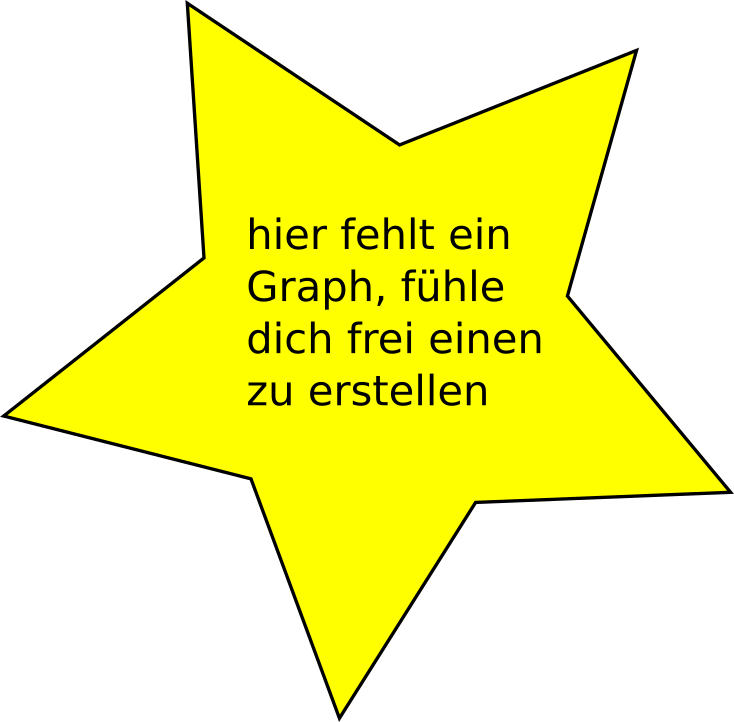
\includegraphics[width=0.3\linewidth]{graphs/dummy}
	 		%				\includegraphics[width=0.7\linewidth]{graphs/plot10_1}
	 		\caption{Konkavität der Wurzelfunktion}
		\end{figure}
		
		Die Wurzelfunktion ist konkav:
		\[ f(\lambda x + (1- \lambda) y) \geq \lambda f(x) + (1-\lambda) f(y) \] 
		
		\[ =   \frac{2c}{m} \sqrt{E_\sigma[\sum_{i,j=1}^{m} \sigma^{(i)} \sigma^{(j)} z^{(i)^T} z^{(j)}} \]
		\[ =   \frac{2c}{m} \sqrt{\sum_{i,j=1}^{m} E_\sigma[ \sigma^{(i)} \sigma^{(j)} z^{(i)^T} z^{(j)}} \]
		\[ =   \frac{2c}{m} \sqrt{[\sum_{i,j=1}^{m} z^{(i)^T} z^{(j)}} \]
		\[ = \frac{2c}{m} \sqrt{spur(k)}, k = (k_{i,j}) = (z^{(i)^T}z^{(j)}) \footnote{Gram-Matrix, Kernel Matrix}\]
		
		
		
				

\end{document}